%
% Modified by Megan Patnott
% Last Change: Jan 18, 2013
%
%%%%%%%%%%%%%%%%%%%%%%%%%%%%%%%%%%%%%%%%%%%%%%%%%%%%%%%%%%%%%%%%%%%%%%%%
%
% Modified by Sameer Vijay
% Last Change: Tue Jul 26 2005 13:00 CEST
%
%%%%%%%%%%%%%%%%%%%%%%%%%%%%%%%%%%%%%%%%%%%%%%%%%%%%%%%%%%%%%%%%%%%%%%%%
%
% Sample Notre Dame Thesis/Dissertation
% Using Donald Peterson's ndthesis classfile
%
% Written by Jeff Squyres and Don Peterson
%
% Provided by the Information Technology Committee of
%   the Graduate Student Union
%   http://www.gsu.nd.edu/
%
% Nothing in this document is serious except the format.  :-)
%
% If you have any suggestions, comments, questions, please send e-mail
% to: ndthesis@gsu.nd.edu
%
%%%%%%%%%%%%%%%%%%%%%%%%%%%%%%%%%%%%%%%%%%%%%%%%%%%%%%%%%%%%%%%%%%%%%%%%


%
% Chapter 6
%

\chapter{Discussion}

Understanding the nature of collective bands in nuclei requires the use of multiple tools. Energies, transition characterization including strengths and multpolarities, and lifetime information are all vital. Combining this data together creates a story to understand the nature ofa given excitation of the band.

\section{Dynamic Symmetries in Nuclei}

Dynamical symmetries are a way to describe physical properties of nuclear systems with explicit analytical form, introduced in the late 1970s \citep{vanisacker99:_symmetries}. One of the notable examples of a dynamical system is that of the interacting boson model (IBM). The standard interacting boson triangle of symmetries is in Figure \ref{fig:castentriangle}. The three corners represent the limits of a vibrator, rotor, and $\gamma$-soft (or $\gamma$-unstable) models of nuclei. A nucleus can, in principle, rest anywhere within the triangle. The points E(5) and X(5) are phase transition points, coming as an extension of IBM. The concept was introduced by Iachello in 2000 \citep{iachello00:_x5}, with first evidence noted later that year \citep{casten00:_x5}. Properties of these transition nuclei can be described analytically, predicting differences in energies of excited states in the nucleus located at critical points, for example \citep{iachello01:_x5}.

The predicted ratios for the X(5) critical point symmetry agree well with the ratios for $^{154}$Gd \citep{tonev04:_154gd}. A more stringent test of the X(5) predictions, the absolute B(E2) values, agree and classify $^{154}$Gd as an X(5) nucleus. Importantly, one of the assumptions Iachello made when developing these critical point symmetries was shape coexistence between the two lowest $0^+$ states in the nucleus. The IBM predicted the deformations of these two excited $0^+$ states will become similar as the deformed limit is reached\citep{werner08:_x5}. While $^{156}$Gd has also been examined through the lens of the interacting boson model, it is a rotor in the axially-deformed limit.

\begin{figure}[t]
    \centering
    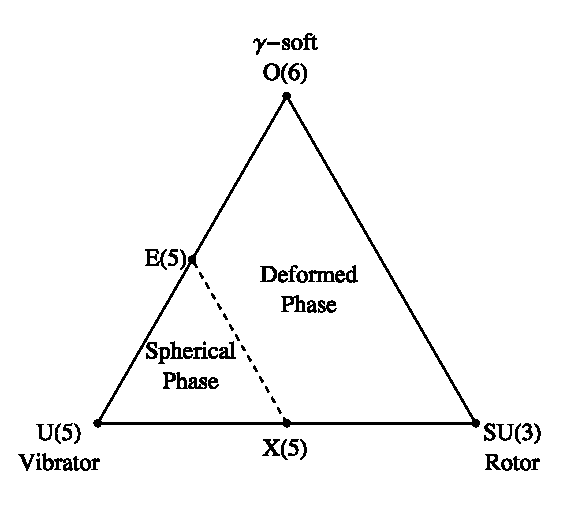
\includegraphics[scale=1]{Discussion/CastenTriangle.eps}
    \caption{The interacting boson model symmetry triangle. The critical point symmetries described by Iachello\citep{iachello00:_x5} are marked.}
    \label{fig:castentriangle}
\end{figure}

\section{Dynamic Moments of Inertia}
\label{sec:Dynamic}

"Identical bands" in neighboring nuclei are a phenomenon that was highlighted in the 1990s by Baktash \citep{baktash95:_dynamic_inertia}. These "identical bands" indicate identical moments of inertia in two different nuclei, pointing to the common origin of the excitation bands. Baktash\citep{baktash95:_dynamic_inertia} defines two different moments of inertia: kinematic ($\mathscr{J}^{(1)}$) and dynamic ($\mathscr{J}^{(2)}$), specifically identifying $\mathscr{J}^{(2)}$ as being identical in both bands, indicating identical origins. These moments of inertia can be approximated for rotational bands as 
\begin{equation}
    \begin{split}
        \mathscr{J}^{(1)}\equiv I/\omega \approx 2I/E_{\gamma} \\
        \mathscr{J}^{(2)}\equiv (d^2E/dI^2)^{-1} = dI/d\omega \approx 4/\delta E_{\gamma}
    \end{split}
\end{equation}
where $I$ is the spin of the level being depopulated, $E_{\gamma}$ is the energy of the gamma depopulating level $I$, $\delta E_{\gamma}$ is the difference between two separate energies of gamma transitions, and $\omega$ us the rotational frequency such that 
\begin{equation}
    \hbar \omega(I) =dE_{I}/dI \approx \left[E(I+1)-E(I-1)\right]/2 = E_{\gamma}(I+1)/2
\end{equation}
As $\mathscr{J}^{(2)}$ is a derivative of the spin, it eliminates any single particle component of the aligned angular momentum, making it a better indicator if the collective properties of the band. There is still a slowly changing component that is seen with increasing spin.

Baktash discussed the identical band phenomenon between two different nuclei of identical origin. They have been used to compare bands within the same nucleus, giving insight into the nature of the collective excitations in deformed nuclei \citep{aprahamian18:_156gd}. Combining the dynamic moment of inertia with measures of the $\rho^2$ of E0 transitions can give further insight into the nuclear matrix element. The E0 matrix element has two components, the overlap of the wave function and matrix elements connecting the wave function, seen as a change in the radius of the nucleus between two states of the same $J^{\pi}$. Comparing the dynamic moments of inertia of the two bands involved in an E0 transition can aid in examining the strength of the nuclear overlap.

To examine the structure of the bands seen in this experiment, the dynamic moments of inertia can be compared. This is usually done with higher spins, but examination at lower spins can allow for more bands to be compared. The energy difference tracks linearly, with the slope being directly correlated to the moment of inertia of the band, as seen in Figures \ref{fig:154_Dynamic}, \ref{fig:154_Dynamic0}, \ref{fig:156_Dynamic}, and \ref{fig:156_Dynamic0}. The slopes of these bands are summarized in Tables \ref{tab:154_Dynamic} and \ref{tab:156_Dynamic}. Slopes will vary with spin, and slopes with an error had enough points to calculate the error on the slope based on the fit. Those without error had only two points or, in the case of the second excited $2^+$ band, one point and the origin. These points each require two levels of the band to be known for calculation. The intercept was left to float, but not included, as it was in agreement with 0 in all cases where error could be calculated.

\section{$^{154}$Gd Results}
\label{sec:154_Discussion}
In Chapter \ref{chap:154Gd}, the results of this work on the nucleus $^{154}$Gd were detailed. From the singles data multipole assignments were confirmed for two transitions, conversion coefficients were measured for 30 transitions, and $\delta$ was measured for one. A new transition, from $5^-_{0^-}\rightarrow 6^+_{gs}$ was seen. Five pure E0 transitions were measured via coincidence (Table \ref{tab:154Gd_0_to_0}), with two of these transitions having been measured for the first time in this work ($0^+_6\rightarrow 0^+_2$ and $0^+_7\rightarrow 0^+_3$). None of these $0^+$ states had lifetimes, but the $q_K^2(E0/E2)$ value was calculated for all the transitions (Table \ref{tab:154Gd_E0_0}).

A total of 22 $J^{\pi}\rightarrow J^{\pi}$ transitions were measured for $2^+$ (Table \ref{tab:154Gd_2_to_2}), $4^+$ (Table \ref{tab:154Gd_4_to_4}), and $6^+$ (Table \ref{tab:154Gd_6_to_6}) states, 11 of these transitions for the first time. Of these 22 transitions, 11 have conversion coefficients indicating evidence of E0 components. Four of these transitions had known $\delta$ mixing ratios, allowing for the calculation of $\epsilon$, the E0/E2 mixing ratio (Table \ref{tab:154Gd_E0_d}), and in two cases with known lifetimes, the nuclear strength parameter $\rho^2(E0)$. For the rest of the transitions, $\delta$ was assumed to be 1, so $q^2\alpha(E2)$ and B(E0) ratios were calculated for transitions depopulating the same level (Tables \ref{tab:154Gd_E0} and \ref{tab:154Gd_BE0_Comp}). Combining these ratios with the dynamic moments of inertia can give some insight into the strength of $\rho^2(E0)$.

\begin{figure}[!]
    \begin{subfigure}{\textwidth}
    \centering
    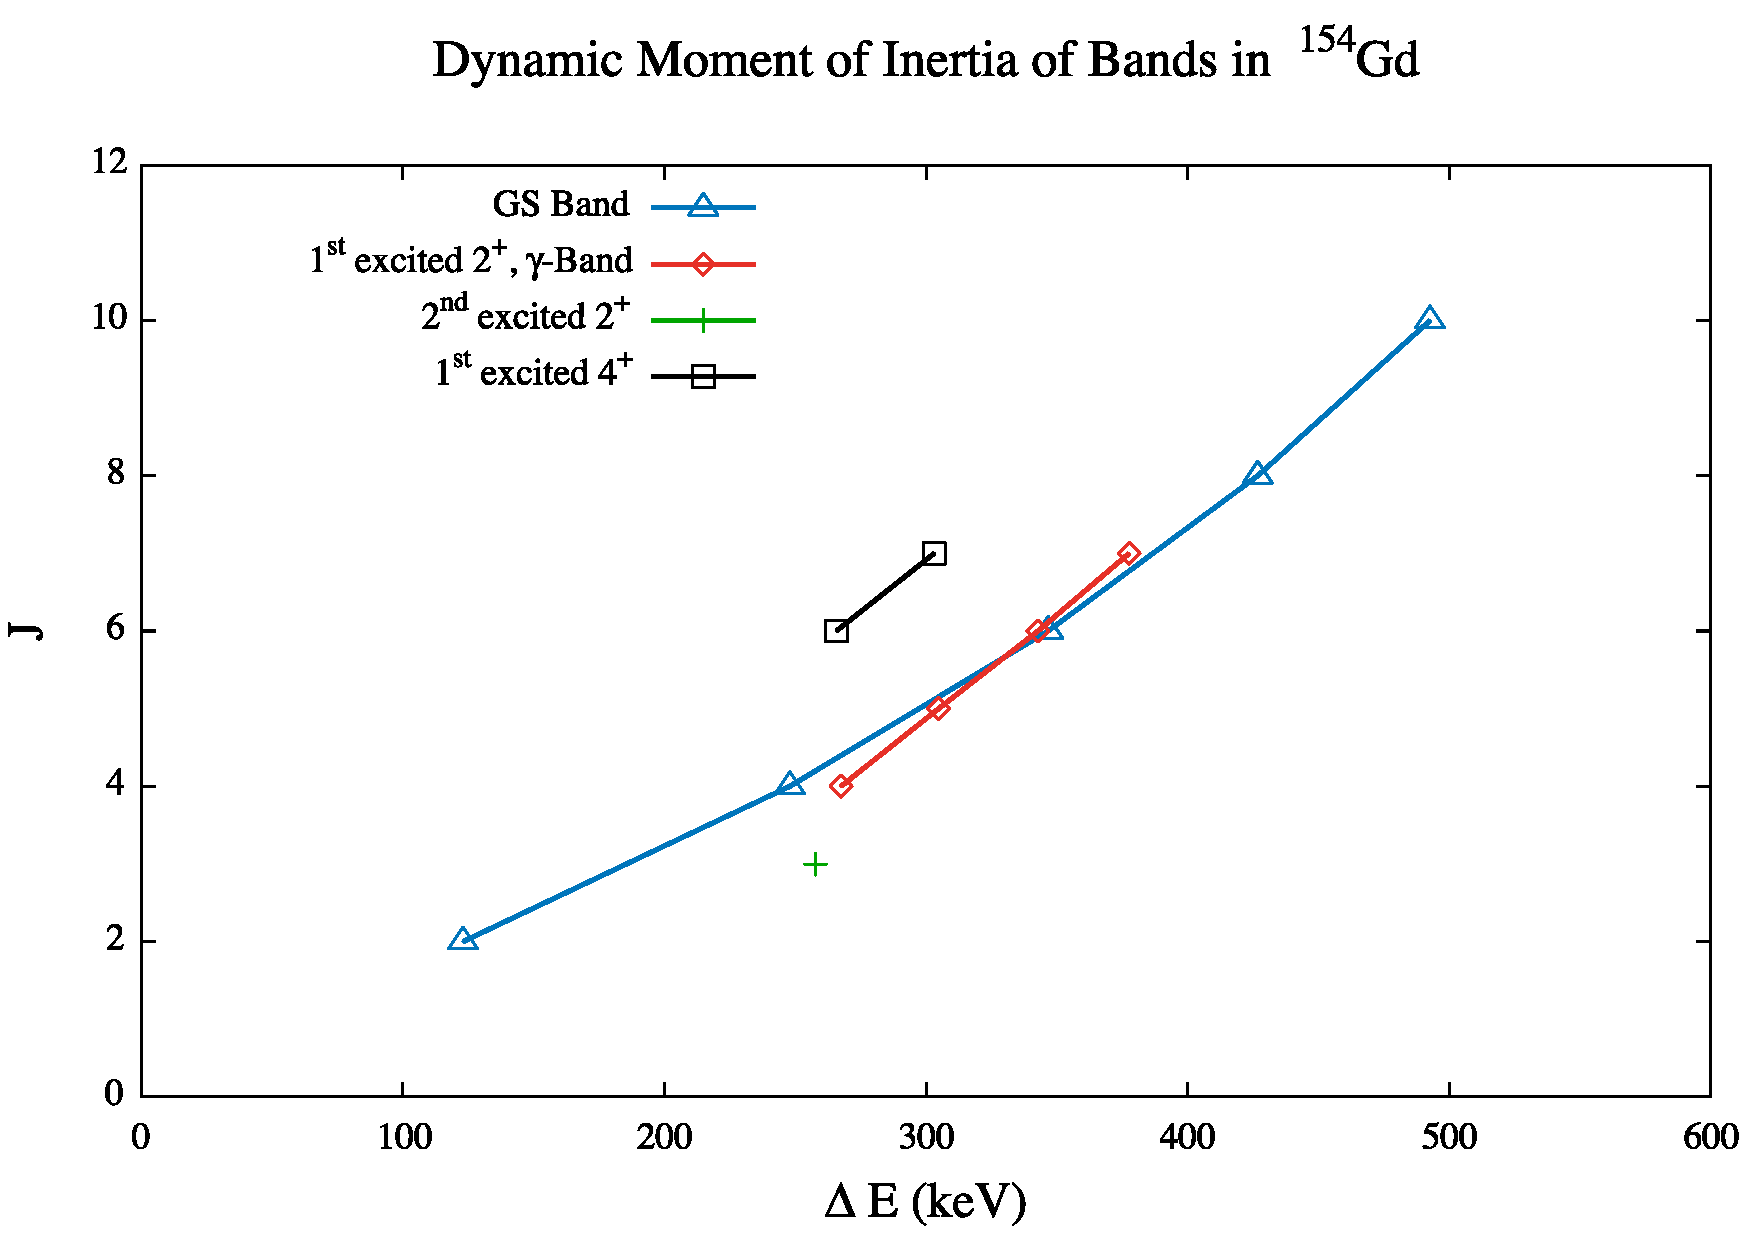
\includegraphics[scale=0.4]{Discussion/154_Dynamic.pdf}
    \caption*{(a)}
    \end{subfigure}
    \begin{subfigure}{\textwidth}
    \centering
    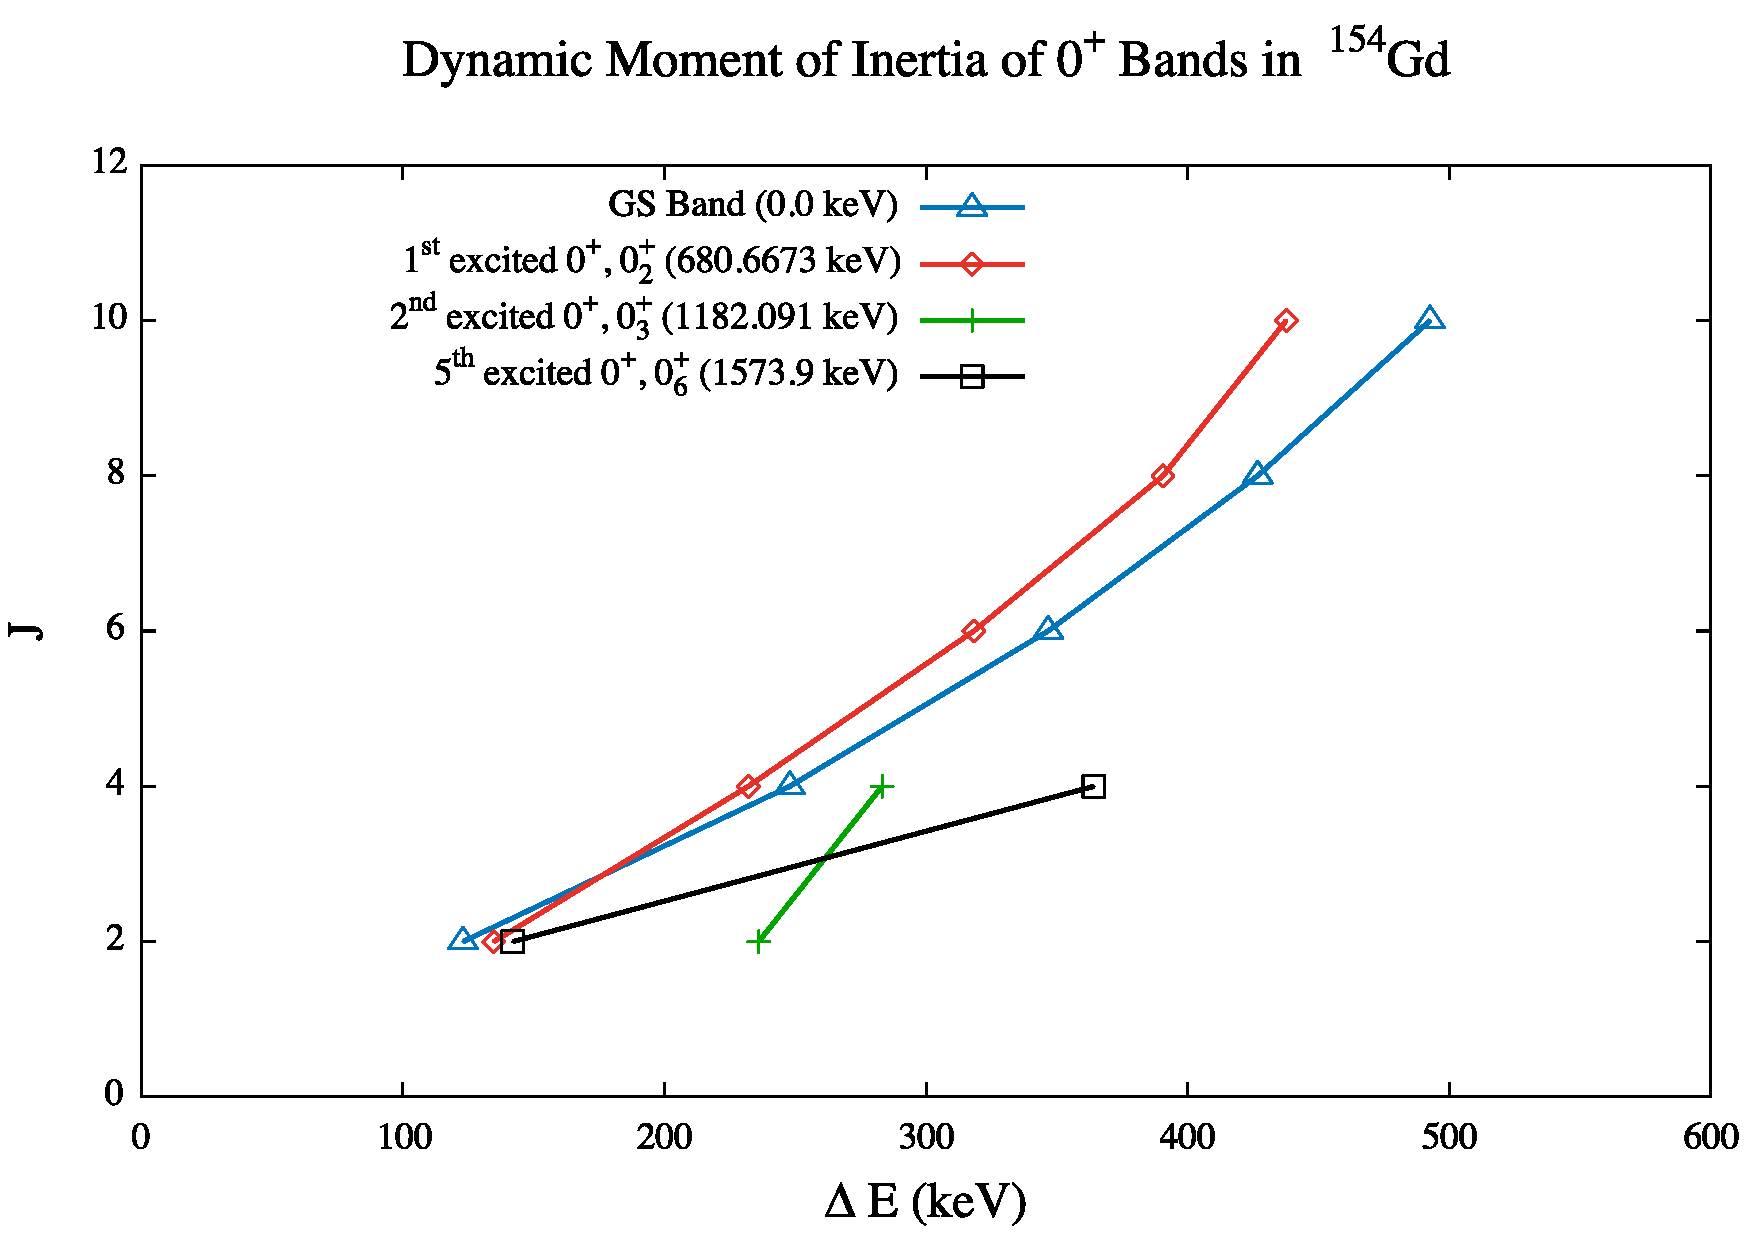
\includegraphics[scale=0.4]{Discussion/154_Dynamic0.pdf}
    \caption*{(b)}
    \end{subfigure}
    \caption{(a) The dynamic moments of inertia of the ground state, $K=2^+_1$ and $K=4^+_1$ bands. As is seen visually and with the slopes, the ground state band and the $\gamma$ band have similar moments of inertia and the $K=2^+_1$ and $K=4^+_1$ bands have identical moments of inertia. (b) The dynamic moments of inertia of the four $0^+$ bands seen in the experiment. The ground state band and the first excited $0^+$ band have very similar moments of inertia, while the second and fifth $0^+$ bands differ greatly.}
    \label{fig:154_Dynamic}
\end{figure}

\begin{figure}[!]
    \centering
    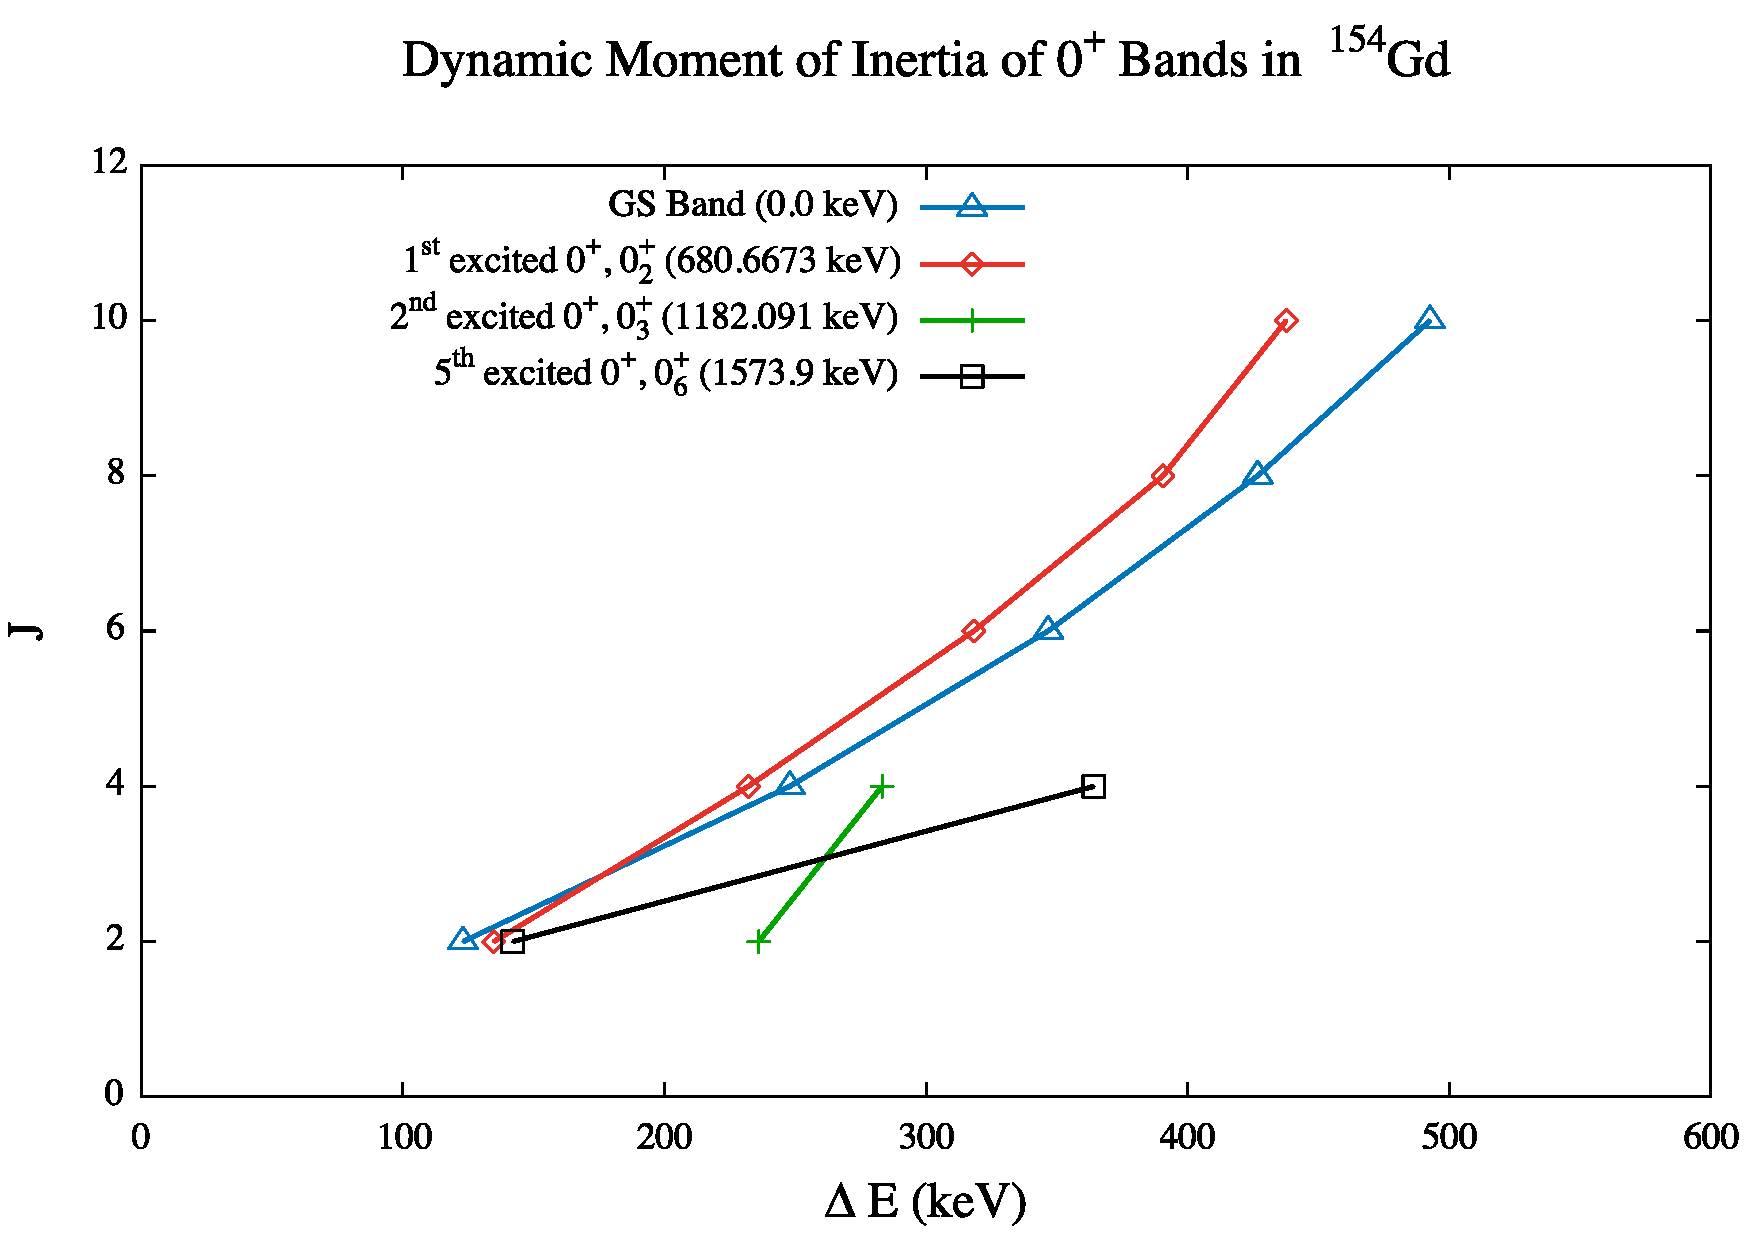
\includegraphics[scale=0.45]{Discussion/154_Dynamic0.pdf}
    \caption{The dynamic moments of inertia of the four $0^+$ bands seen in the experiment. As is seen visually and with the slopes, the ground state band and the first excited $0^+$ band have very similar moments of inertia.}
    \label{fig:154_Dynamic0}
\end{figure}

\begin{table}[!]
    \centering
    \caption{Dynamic Moments of Inertia of Bands seen in $^{154}$Gd}
    \begin{tabular}{c|c}
        \toprule
        Band & Moment of Inertia  \\
        \hline
        Ground State & 0.0214 (15) \\
        1st excited $0^+$, $0^+_2$ & 0.0258 (19) \\
        2nd excited $0^+$, $0^+_3$ & 0.0424 \\
        5th excited $0^+$, $0^+_6$ & 0.0090 \\
        1st excited $2^+$, $\gamma$-band & 0.0271 (3) \\
        2nd excited $2^+$ & 0.0155 \\
        1st excited $4^+$ & 0.0267 \\
        \bottomrule
    \end{tabular}
    \\[2pt]
    \footnotesize
    \label{tab:154_Dynamic}
    Table \ref{tab:154_Dynamic}: List of the moments of inertia of the bands seen in $^{154}$Gd in this experiment. The moment of inertia is the slope in a least-squares linear regression. Those without error only had one or two points of energy difference, so the standard deviation of the slope could not be calculated. The ground state band the the first excited $0^+$ band agree within two standard deviations.
\end{table}

The $\gamma$-band, seen in Figure \ref{fig:154_Dynamic} is a vibration built on the ground state, leading to a nearly identical dynamic moment of inertia. The $K=4^+$ band has a nearly identical moment of inertia to the $\gamma$-band, indicating it, too, may be a vibration built on the same structure as the ground state. The first excited $0^+$ state $0^+_2$, seen in Figure \ref{fig:154_Dynamic0}, agrees with the $\gamma$-band within $1\sigma$. The variation in the error of slopes has to do with the slow change in $\mathcal{J}^{(2)}$ due to the increase in spin. 

\subsection{$K^{\pi}=0^+_2$, First Excited $0^+$ Band, 680.6673 keV}

The conversion coefficients for the singles and gated data originating from the first excited $0^+$ band are in Tables \ref{tab:154Gd_Single_02_Disc} and \ref{tab:154Gd_02_Gate_Disc}, respectively. The first excited $0^+$ band is the only band with lifetimes and mixing ratios such that $\rho^2$ could be calculated, seen in Table \ref{tab:154Gd_E0_0}. The first excited $0^+$ band has a very similar slope to the ground state band, as seen both in Figure \ref{fig:154_Dynamic0} and Table \ref{tab:154_Dynamic}, indicating similar moments of inertia. Lifetimes beyond the $4^+$ state are unknown, so the $\rho^2$ value cannot be calculated for the $6^+$ state, but could be calculated for the $2^+$ and $4^+$ states. The similarity in the dynamic moment of inertia, coupled with the large $\rho^2$ values, indicate a $\beta$-vibration. The $\gamma$-vibration band dynamic moment of inertia behaves very similarly to the ground state in much the same way, also favoring this interpretation. 

\begin{table}
    \centering
    \caption{$^{154}$Gd $K_i=0^+_2$ Internal Conversion Coefficients from Singles}
    \label{tab:154Gd_Single_02_Disc}
\begin{ThreePartTable}
    \begin{subtable}{\textwidth}
        \caption{}
    \begin{tabular}{c|c|c|c|c|c|c}
        \toprule
        $E$ (keV)	&	$J^{\pi}	\rightarrow	J^{\pi}$	&	$E_i$ (keV)	&	$E_f$ (keV)	&	$T_{1/2}$ (fs)	&	Multipolarity	&	$\delta$\\
        \hline
        557.58	&	$0^+_{0^+_2}	\rightarrow	2^+_{gs}$	&	680.6673	&	123.0709	&	4560	&	E2	&		\\
        \hline
        444.19	&	$2^+_{0^+_2}	\rightarrow	4^+_{\gamma}$	&	815.4917	&	370.9998	&	6400	&	E2	&		\\
        \hline
        693.47	&	$2^+_{0^+_2}	\rightarrow	2^+_{gs}$	&	815.4917	&	123.0709	&	6400	&	E2+M1+E0	&	7.5 (4)	\\
        \hline
        232.44	&	$4^+_{0^+_2}	\rightarrow	2^+_{0^+_2}$	&	1047.592	&	815.4917	&	7600	&	E2	&	\\
	    &				&		&		&		&		& \\
	    \hline
        329.49	&	$4^+_{0^+_2}	\rightarrow	6^+_{gs}$	&	1047.592	&	717.662	&	7600	&	E2	&	\\
        \hline

        676.70	&	$4^+_{0^+_2}	\rightarrow	4^+_{gs}$	&	1047.592	&	370.9998	&	7600	&	E0+M1+E2	&	+2.9 (4)	\\
        \hline
        924.85	&	$4^+_{0^+_2}	\rightarrow	2^+_{gs}$	&	1047.592	&	123.0709	&	7600	&	E2	&	\\
        \hline        
        610.71	&	$8^+_{0^+_2}	\rightarrow	8^+_{gs}$	&	1756.49	&	1144.44	&		&	E0+M1+E2	&	-0.69 (14)	\\
	    &				&		&		&		&		&	\\
	    \bottomrule
    \end{tabular}
    \end{subtable}
    \end{ThreePartTable}
\end{table}
\begin{table}
    \ContinuedFloat
    \begin{subtable}{\textwidth}
    \end{subtable}
    \begin{ThreePartTable}
    \begin{subtable}{\textwidth}
        \caption{}
        \begin{tabular}{c|c|c|c|c|c|c}
            \toprule
            $E$ (keV) & Shell &	$\alpha$ (This Work)	&	$\alpha$  (Theory)\citep{kibedi08:_BRICC}	&	$\alpha$ (Spits)\citep{spits96:_154gd} & $\alpha$ (Gono)\citep{gono74:_154gd_e0}	& $\epsilon^2$ (This Work)	\\
            \hline
            557.58	& K &	0.0486	(42) (6)	&	0.00864 (12)	&	0.009 (1) & 0.0091 (16)	& \\
            \hline
            444.19	& K &	0.0525	(32) (6)	&	0.01543 (22)	&	0.014 (1)&	\\
            \hline
            693.47	& K &	0.0017	(2) (1)	&	0.00522 (8)	&	0.0421 (4) &	\\
            \hline
            232.44	& K &	0.287	(103) $^{+83}_{-82}$	&	0.0982 (14)	&	0.100 (8)	& \\
            &	LM &		0.0450	(46) (13)	&	0.0288 (4)	&	&	\\
            \hline
            329.49	 & K &	0.1573	(89) (17)	&	0.0352 (5)	&	0.034 (3)	&\\
            \hline
            676.70	& K &	0.0283	(4) (10)	&	0.00593 (17)	&	0.0460 (46) & 0.040 (7)	& 0.1762 (244) (62)\\
            \hline
            924.85	& K &	0.0033	(9) (1)	&	0.00273 (4)	&	0.0031 (1)	&\\
            \hline
            610.71	& K &	0.0258	(10) (7)	&	0.0110 (6)	& &	0.053 (7)	& 0.0250 (52) (7)\\
            		& L &	0.0167	(9) (4)	&	0.00158 (7)	&	&	& 0.0227 (48) (5) \\
            \bottomrule
        \end{tabular}
        \end{subtable}

        \makeatletter\def\TPT@hsize{}\makeatletter
        
        \begin{tablenotes}[para,flushleft]
            Table \ref{tab:154Gd_Single_02_Disc}: A list of conversion coefficients from $^{154}$Gd, originating in the $K_i=0^+_2$ band. Table (a) lists transition information. Multipolarities and mixing ratios were taken from the nuclear data sheets\citep{reich09:_nds_154}. Table (b) lists the conversion coefficients. Unless otherwise stated, the $\alpha$ values are $\alpha_K$. An angular distribution correction has been applied based on multipolarities for pure transitions, and those with known mixing ratios. For transitions with an E0 component, the correction was applied assuming just the M1 and E2 components. The theory value is based on the listed multipolarity, also neglecting the E0 component in those cases. The $\epsilon^2$ values listed are for transitions with an E0 component possible, and a large enough $\alpha_{exp}$. The first error is statistical, the second is systematic. Numbers are compared with Spits et al.\citep{spits96:_154gd} and Gono et al.\citep{gono74:_154gd_e0}. The bands for each level are listed as subscripts.
        \end{tablenotes}
\end{ThreePartTable}
\end{table}


\begin{landscape}
\begin{table}
    \centering
    \caption{$J^{\pi}\rightarrow J^{\pi}$ Transitions for $K_i=0^+_2$ in $^{154}$Gd}
    \label{tab:154Gd_02_Gate_Disc}
\begin{ThreePartTable}
    \begin{subtable}{\textwidth}
        \caption{}
    \begin{tabular}{c|c|c|c|c|c}
        \toprule
        $E_i$ (keV)	& $J^{\pi}_i$ &	$E_f$ (keV)	& $J^{\pi}_f$ & $E$ (keV)	&	Gate \\
        \hline
        815.4917 & $2^+_{0^+_2}$ & 123.0709 & $2^+_{gs}$ & 692.4205 & 123.0706\\ \hline
        1047.592 & $4^+_{0^+_2}$ & 370.9998 & $4^+_{gs}$ &  676.593 & 247.9288 \\\hline
        1365.878 & $6^+_{0^+_2}$ & 717.662 & $6^+_{gs}$ & 648.3 & 346.643 \\
	    \bottomrule
    \end{tabular}
    \end{subtable}
    \end{ThreePartTable}
\end{table}
\begin{table}
    \centering
    \ContinuedFloat
    \begin{subtable}{\textwidth}
    \end{subtable}
    \begin{ThreePartTable}
    \begin{subtable}{\textwidth}
        \begin{tabular}{c|c|c|c|c|c|c}
            \multicolumn{7}{c}{TABLE 6.3 (CONTINUED)} \\
            \multicolumn{7}{c}{(b)} \\
            \toprule
            & \multicolumn{5}{c|}{$\alpha$}	& 	\\ 
             &	& \multicolumn{2}{c|}{Theory\citep{kibedi08:_BRICC}}	& & 	\\ 
            $E_i$ (keV)	&This Work	& $\alpha$(M1) & $\alpha$(E2) &	Spits\citep{spits96:_154gd} & Gono\citep{gono74:_154gd_e0} & $\epsilon^2$ (This Work)	\\
            \hline
            815.4917 &  0.0430 (3)(9) & 0.00952 (14) & 0.00516 (8) &  0.0421 (4) & & 1.9233 (1035)(402)\\ \hline
            1047.592 & 0.0550 (2)$^{+12}_{-11}$ & 0.01007 (15) & 0.00544 (8) & 0.0460 (46) & 0.040 (7) & 0.4274 (590)$^{+93}_{-85}$\\
            &   0.0131 (1)(3) & 0.001384 (20) & 0.000870 (13) & & & 0.1108 (153)(25)\\ \hline
            1365.878  & 0.0778 (4)(16) & 0.01120 (16) & 0.00601 (9) & & 0.039 (7) & 0.1017 (206)(21)\\
            \bottomrule
        \end{tabular}
        \end{subtable}

        \makeatletter\def\TPT@hsize{}\makeatletter
        
        \begin{tablenotes}[para,flushleft]
            Table \ref{tab:154Gd_02_Gate_Disc}: A list of conversion coefficients from $^{154}$Gd for $J^{\pi}\rightarrow J^{\pi}$ transitions for $K_i=0^+_2$ seen in the gated data. The first error is statistical, the second is systematic. Numbers are compared with theoretical K-shell conversion coefficients for M1 and E2 transitions, as well as results from Spits et al.\citep{spits96:_154gd} and Gono et al.\citep{gono74:_154gd_e0}. The $\epsilon^2$ values listed are for transitions with a large enough $\alpha_{exp}$ to indicate an E0 component. All coefficients are K-electrons, except for the transition from 1047 keV. The second value is the LM peak.
        \end{tablenotes}
\end{ThreePartTable}
\end{table}
\end{landscape}


\subsection{$K^{\pi}=0^+_3$, Second Excited $0^+$ Band, 1182.091 keV}

The conversion coefficients for the gated data originating from the second excited $0^+$ band are in Table \ref{tab:154Gd_03_Gate_Disc}. All of the measurements from the $K=0^+_3$ band were limits, and connected to either the $0^+_2$ band or the $\gamma$-band. All the transitions were measured with two different gates. The $2^+$ state transitions only had lower limits, with the lower limit on the $\gamma$-band indicating an E0 component. For the $4^+$ state transitions, the limits were upper limits. The upper limit to the $0^+_2$ transition indicated little to no E0 component, while the upper limit on the transition to the $\gamma$-band allows for a larger E0 component. The transitions, in agreement with Table \ref{tab:154Gd_BE0_Comp}, indicate the $0^+_3$ band favors populating the $\gamma$-band. This band also has a much larger dynamic moment of inertia, compared to the ground state, first excited $0^+$ state and $\gamma$-bands. None of the transitions examined have known mixing ratios, so the $q^2$ and $\alpha q^2$ can be found in Tables \ref{tab:154Gd_E0} and \ref{tab:154Gd_E0_0}. 

This band is a possible candidate for shape coexistence. Although the energy would be reasonable for a $\beta-\beta$ vibration if the 680 keV band is the $\beta$ vibration, one would expect a strong E0 transition to that band, which does not appear.

\begin{landscape}
    \footnotesize
    \begin{longtable}{>{\footnotesize}c|>{\footnotesize}c|>{\footnotesize}c|>{\footnotesize}c|>{\footnotesize}c|>{\footnotesize}c|>{\footnotesize}c|>{\footnotesize}c|>{\footnotesize}c|>{\footnotesize}c|>{\footnotesize}c}
        \caption{$J^{\pi}\rightarrow J^{\pi}$ Transitions for $K_i=0^+_3$ in $^{154}$Gd}
        \label{tab:154Gd_03_Gate_Disc}\\
        \toprule
        &	& & & 	&  &	& \multicolumn{2}{>{\footnotesize}c|}{Theory\citep{kibedi08:_BRICC}}	& 	\\ 
        $E_i$ (keV)	& $J^{\pi}_i$ &	$E_f$ (keV)	& $J^{\pi}_f$ & $E$ (keV)	&	Gate &		$\alpha$ (This Work)	& $\alpha$(M1) & $\alpha$(E2) &	$\alpha$ (Spits)\citep{spits96:_154gd} & $\epsilon^2$ (This Work)\\
        \hline
        \endfirsthead
        \caption[]{$J^{\pi}\rightarrow J^{\pi}$ Transitions for $K_i=0^+_3$ in $^{154}$Gd}\\
        \toprule
        &	& & &	&  &	& \multicolumn{2}{>{\footnotesize}c|}{Theory\citep{kibedi08:_BRICC}}	&	\\ 
        $E_i$ (keV)	& $J^{\pi}_i$ &	$E_f$ (keV)	& $J^{\pi}_f$ & $E$ (keV)	&	Gate &		$\alpha$ (This Work)	& $\alpha$(M1) & $\alpha$(E2) &	$\alpha$ (Spits)\citep{spits96:_154gd} & $\epsilon^2$ (This Work)\\
        \hline
	    \endhead
	    \endfoot
        \multicolumn{11}{p{1.4\textwidth}}{Table \ref{tab:154Gd_03_Gate_Disc}: A list of conversion coefficients from $^{154}$Gd for $J^{\pi}\rightarrow J^{\pi}$ transitions for $K_i=0^+_3$ seen in the gated data. The first error is statistical, the second is systematic. Numbers are compared with theoretical K-shell conversion coefficients for M1 and E2 transitions, as well as results from Spits et al.\citep{spits96:_154gd}. The $\epsilon^2$ values listed are for transitions with a large enough $\alpha_{exp}$, and assumed to be pure E2 transitions, to give a minimum $\epsilon^2$. For $\alpha_{exp}$ that are upper limits and $0^+\rightarrow 0^+$ transitions, $\epsilon^2$ is not listed. All coefficients are K-electrons.}
        \endlastfoot
        1182.091 & $0^+_3$ & 680.6673 & $0^+_2$ &  501.427 & 557.581 & $>0.0283$ & 0.0213 (3) & 0.01126 (16) & $>0.2$ & \\\hline
        1418.16 & $2^+_{0^+_3}$ & 815.4917 & $2^+_{0^+_2}$ & 602.688 &  692.4205 & $>0.0125$ & 0.01343 (19) & 0.00715 (10) & 0.025 (3)  & $>0.0054$\\
        &  & &  &  & 444.4924 & $>0.0093$ &  & & & $>0.0022$\\ \hline
        1418.16 &  $2^+_{0^+_3}$ & 996.2568 &  $2^+_{\gamma}$ & 421.893 & 873.1834 & $>0.0367$ & 0.0332 (5) & 0.01170 (25) & 0.114 (16) & $>0.0250$\\
        &  & &  &  & 625.2556 & $>0.0463$ & & & & $>0.0346$\\ \hline
        1701.39 & $4^+_{0^+_3}$ & 1047.592 & $4^+_{0^+_2}$ & 653.7 & 676.593 & $<0.0093$ & 0.01097 (16) & 0.00590 (9) & 0.0220 (62)  & \\
        &  & &  &  & 924.55 & $<0.0301$ & & & &\\ \hline
        1701.39 & $4^+_{0^+_3}$ & 1263.778 & $4^+_{\gamma}$ & 437.612 & 892.775 & $<0.0585$ & 0.0302 (5) & 0.01605 (23) &  & \\
        &  & &  &  & 1140.702 & $<0.0511$ & & &  & \\ 
        \bottomrule
    \end{longtable}
\end{landscape}

\subsection{$K^{\pi}=0^+_6$, Fifth Excited $0^+$ Band, 1573.9 keV}

The conversion coefficients for the singles and gated data originating from the fifth excited $0^+$ band are in Tables \ref{tab:154Gd_Single_06_Disc} and \ref{tab:154Gd_06_Gate_Disc}, respectively. Transitions between the $0^+_6$ band and the $0^+_2$ and $0^+_3$ bands could be seen in the gates, specifically for the $0^+$ states. $\rho^2$ could not be calculated due to a lack of lifetime, but the two transitions could be compared, in Table \ref{tab:154Gd_BE0_Comp}, indicating a stronger connection to the $0^+_3$ band. Comparisons between the $0^+_2$ and $\gamma$-band were also done using the $2^+$ state, generally indicating a stronger connection to the $\gamma$-band than the $0^+_2$ band. None of the transitions examined have known mixing ratios, so the $q^2$ and $\alpha q^2$ can be found in Tables \ref{tab:154Gd_E0} and \ref{tab:154Gd_E0_0}. The fifth excited $0^+$ band has the smallest slope of all the bands looked at in this nucleus, the strongly different moment of inertia gives an indication this band is likely not built on the $\gamma$-band or $0^+_2$ band.

\begin{table}
    \centering
    \caption{$^{154}$Gd $K_i=0^+_6$, Internal Conversion Coefficients from Singles}
    \label{tab:154Gd_Single_06_Disc}
\begin{ThreePartTable}
    \begin{subtable}{\textwidth}
        \caption{}
    \begin{tabular}{c|c|c|c|c|c|c}
        \toprule
        $E$ (keV)	&	$J^{\pi}	\rightarrow	J^{\pi}$	&	$E_i$ (keV)	&	$E_f$ (keV)	&	$T_{1/2}$ (fs)	&	Multipolarity	&	$\delta$\\
        \hline
        416.79	&	$4^+_{0^+_6}	\rightarrow	3^+_{2^+}$	&	2080.23	&	1660.903	&		&	(M1)	&	\\
        \bottomrule
    \end{tabular}
    \end{subtable}
    \end{ThreePartTable}
\end{table}
\begin{table}
    \ContinuedFloat
    \begin{subtable}{\textwidth}
    \end{subtable}
    \begin{ThreePartTable}
    \begin{subtable}{\textwidth}
        \caption{}
        \begin{tabular}{c|c|c|c|c|c}
            \toprule
            $E$ (keV) & Shell &	$\alpha$ (This Work)	&	$\alpha$  (Th)\citep{kibedi08:_BRICC}	&	$\alpha$ (Spits)\citep{spits96:_154gd} & $\alpha$ (Gono)\citep{gono74:_154gd_e0}		\\
            \hline
            416.79	 & K &	0.0334	(47) (6)	&	0.03442 (5)	&	\\
            \bottomrule
        \end{tabular}
        \end{subtable}
        \begin{tablenotes}[para]
            Table \ref{tab:154Gd_Single_06_Disc}: A list of conversion coefficients from $^{154}$Gd, originating in the $K_i=0^+_6$ band. Table (a) lists transition information. Multipolarities and mixing ratios were taken from the nuclear data sheets\citep{reich09:_nds_154}. Table (b) lists the conversion coefficients. Unless otherwise stated, the $\alpha$ values are $\alpha_K$. An angular distribution correction has been applied based on multipolarities for pure transitions, and those with known mixing ratios. The first error is statistical, the second is systematic. Numbers are compared with Spits et al.\citep{spits96:_154gd} and Gono et al.\citep{gono74:_154gd_e0} The starred value was used as an absolute calibration of the conversion electron detector in the Gono work. The bands for each level are listed as subscripts.
        \end{tablenotes}
\end{ThreePartTable}
\end{table}


\begin{landscape}
    \footnotesize
    \begin{longtable}{>{\footnotesize}c|>{\footnotesize}c|>{\footnotesize}c|>{\footnotesize}c|>{\footnotesize}c|>{\footnotesize}c|>{\footnotesize}c|>{\footnotesize}c|>{\footnotesize}c|>{\footnotesize}c|>{\footnotesize}c}
        \caption{$J^{\pi}\rightarrow J^{\pi}$ Transitions for $K_i=0^+_6$ in $^{154}$Gd}
        \label{tab:154Gd_06_Gate_Disc}\\
        \toprule
        &	& & & 	&  &	& \multicolumn{2}{>{\footnotesize}c|}{Theory\citep{kibedi08:_BRICC}}	& 	\\ 
        $E_i$ (keV)	& $J^{\pi}_i$ &	$E_f$ (keV)	& $J^{\pi}_f$ & $E$ (keV)	&	Gate &		$\alpha$ (This Work)	& $\alpha$(M1) & $\alpha$(E2) &	$\alpha$ (Spits)\citep{spits96:_154gd} & $\epsilon^2$ (This Work)\\
        \hline
        \endfirsthead
        \caption[]{$J^{\pi}\rightarrow J^{\pi}$ Transitions for $K_i=0^+_6$ in $^{154}$Gd}\\
        \toprule
        &	& & &	&  &	& \multicolumn{2}{>{\footnotesize}c|}{Theory\citep{kibedi08:_BRICC}}	& 	\\ 
        $E_i$ (keV)	& $J^{\pi}_i$ &	$E_f$ (keV)	& $J^{\pi}_f$ & $E$ (keV)	&	Gate &		$\alpha$ (This Work)	& $\alpha$(M1) & $\alpha$(E2) &	$\alpha$ (Spits)\citep{spits96:_154gd} & $\epsilon^2$ (This Work)\\
        \hline
	    \endhead
	    \endfoot
        \multicolumn{11}{p{1.4\textwidth}}{Table \ref{tab:154Gd_06_Gate_Disc}: A list of conversion coefficients from $^{154}$Gd for $J^{\pi}\rightarrow J^{\pi}$ transitions for $K_i=0^+_6$ seen in the gated data. The first error is statistical, the second is systematic. Numbers are compared with theoretical K-shell conversion coefficients for M1 and E2 transitions, as well as results from Spits et al.\citep{spits96:_154gd}. The $\epsilon^2$ values listed are for transitions with a large enough $\alpha_{exp}$, and assumed to be pure E2 transitions, to give a minimum $\epsilon^2$,a lower limit. For $\alpha_{exp}$ that are upper limits, $\epsilon^2$ is not listed. No $\epsilon^2$ is indicated for the $0^+\rightarrow 0^+$ transitions. All coefficients are K-electrons, except for the transition from 1047 keV. The second value is the LM peak.}
        \endlastfoot
        1573.9 & $0^+_6$ & 680.6673 & $0^+_2$ &  893.9 & 557.581 & $>0.0183$ & 0.00510 (8) & 0.00294 (5) & &\\\hline
        1573.9 & $0^+_6$ & 1182.091 & $0^+_3$ & 391.9 &  1059.033 & $>0.0529$ & 0.0402 (6) & 0.0216 (3) & $>0.1$ & \\\hline
        1716.050 & $2^+_{0^+_2}$ & 815.4917 & $2^+_{0^+_2}$ & 900.5583 &  692.4205 & $<0.0105$ & 0.00501 (7) & 0.00289 (4) & &  \\
        & & &  & & 444.4924 & $<0.0531$ & & &  & \\ \hline
        1716.050 & $2^+_{0^+_6}$ & 996.2568 & $2^+_{\gamma}$ & 719.80 & 873.1834 & 0.0113 (46)$^{+33}_{-25}$ & 0.00865 (13) & 0.00472 (7) & & $>0.0066$\\
        &  & &  &  & 625.2556 & 0.0501 (260)$^{+147}_{-113}$ & & &  & $>0.0454$\\ 
        \bottomrule
    \end{longtable}
\end{landscape}

\subsection{$K^{\pi}=0^+_7$, Sixth Excited $0^+$ Band, 1650.3 keV}

The conversion coefficients for the gated data originating from the sixth excited $0^+$ band are in Table \ref{tab:154Gd_03_Gate_Disc}. Transitions between the $0^+_7$ band and the $0^+_2$ and $0^+_3$ bands could be seen in the gates, specifically for the $0^+$ states. $\rho^2$ could not be calculated due to a lack of lifetime, but the two transitions could be compared, in Table \ref{tab:154Gd_BE0_Comp}, indicating a stronger connection to the $0^+_3$ band. Comparisons between the $0^+_2$ and $\gamma$-band were also done using the $2^+$ state, generally indicating a stronger connection to the $\gamma$-band than the $0^+_2$ band, although with this ratio being a limit, this could be untrue. None of the transitions examined have known mixing ratios, so the $q^2$ and $\alpha q^2$ can be found in Tables \ref{tab:154Gd_E0} and \ref{tab:154Gd_E0_0}. This band did not have enough information to calculate the dynamic moment of inertia, hence its omission from Figure \ref{fig:154_Dynamic0} and Table \ref{tab:154_Dynamic}.

Although the dynamic moment of inertia might indicate otherwise, this band is a prime candidate for the $0^+$ component of the $\gamma-\gamma$ vibration. The energy of the band is correct, and nearly the same as the $4^+$ band at 1645 keV. The large errors on the conversion coefficients do not rule out E2 transitions to the $\gamma$ vibration band. E2 transitions between the bands would be expected if it were a $\gamma-\gamma$ vibration.

\begin{landscape}
    \footnotesize
    \begin{longtable}{>{\footnotesize}c|>{\footnotesize}c|>{\footnotesize}c|>{\footnotesize}c|>{\footnotesize}c|>{\footnotesize}c|>{\footnotesize}c|>{\footnotesize}c|>{\footnotesize}c|>{\footnotesize}c|>{\footnotesize}c}
        \caption{$J^{\pi}\rightarrow J^{\pi}$ Transitions for $K_i=0^+_7$ in $^{154}$Gd}
        \label{tab:154Gd_07_Gate_Disc}\\
        \toprule
        &	& & & 	&  &	& \multicolumn{2}{>{\footnotesize}c|}{Theory\citep{kibedi08:_BRICC}}	& 	\\ 
        $E_i$ (keV)	& $J^{\pi}_i$ &	$E_f$ (keV)	& $J^{\pi}_f$ & $E$ (keV)	&	Gate &		$\alpha$ (This Work)	& $\alpha$(M1) & $\alpha$(E2) &	$\alpha$ (Spits)\citep{spits96:_154gd}& $\epsilon^2$ (This Work)\\
        \hline
        \endfirsthead
        \caption[]{$J^{\pi}\rightarrow J^{\pi}$ Transitions for $K_i=0^+_6$ in $^{154}$Gd}\\
        \toprule
        &	& & &	&  &	& \multicolumn{2}{>{\footnotesize}c|}{Theory\citep{kibedi08:_BRICC}}	& \\ 
        $E_i$ (keV)	& $J^{\pi}_i$ &	$E_f$ (keV)	& $J^{\pi}_f$ & $E$ (keV)	&	Gate &		$\alpha$ (This Work)	& $\alpha$(M1) & $\alpha$(E2) &	$\alpha$ (Spits)\citep{spits96:_154gd}& $\epsilon^2$ (This Work)\\
        \hline
	    \endhead
	    \endfoot
        \multicolumn{11}{p{1.4\textwidth}}{Table \ref{tab:154Gd_07_Gate_Disc}: A list of conversion coefficients from $^{154}$Gd for $J^{\pi}\rightarrow J^{\pi}$ transitions for $K_i=0^+_7$ seen in the gated data. The first error is statistical, the second is systematic. Numbers are compared with theoretical K-shell conversion coefficients for M1 and E2 transitions, as well as results from Spits et al.\citep{spits96:_154gd}. The $\epsilon^2$ values listed are for transitions with a large enough $\alpha_{exp}$, and assumed to be pure E2 transitions, to give a minimum $\epsilon^2$,a lower limit. For $\alpha_{exp}$ that are upper limits, $\epsilon^2$ is not listed. No $\epsilon^2$ is indicated for the $0^+\rightarrow 0^+$ transitions.All coefficients are K-electrons, except for the transition from 1047 keV. The second value is the LM peak.}
        \endlastfoot
        1650.3 & $0^+_7$ & 680.6673 & $0^+_2$ &  970.3 & 557.581 & $>0.0209$ & 0.00419 (6) & 0.00247 (4) & $>0.027$ \\ \hline
        1650.3 & $0^+_7$ & 1182.091 & $0^+_3$ & 468.3 &  1059.033 & $>0.0922$ & 0.0254 (4) & 0.01343 (19) & \\ \hline
        1775.429 & $2^+_{0^+_7}$ & 815.4917 & $2^+_{0^+_2}$ & 960.05 &  692.4205 & $>0.0221$ & 0.00430 (6) & 0.00253 (4) & & $>0.0196$ \\
        &  & & &  & 444.4924 & $>0.0231$ & & &  & $>0.0206$\\ \hline
        1775.429 & $2^+_{0^+_7}$ & 996.2568 & $2^+_{\gamma}$ & 779.165 & 873.1834 & 0.0206 (112)$^{+60}_{-46}$ & 0.00712 (10) & 0.00396 (6) & & $>0.0166$\\
        &  & &  &  & 625.2556 & 0.0745 (521)$^{+217}_{-165}$	& & & & $>0.0705$\\
        \bottomrule
    \end{longtable}
\end{landscape}

\subsection{$K^{\pi}=2^+$, $\gamma$ Band, 996.264 keV}

The conversion coefficients for the singles and gated data originating from the first excited $2^+$ band, the $\gamma$-vibrational band are in Tables \ref{tab:154Gd_Single_gamma_Disc} and \ref{tab:154Gd_gamma_Gate_Disc}, respectively. The $\gamma$ band has a very similar slope to the ground state band, as seen both in Figure \ref{fig:154_Dynamic} and Table \ref{tab:154_Dynamic}, indicating similar moments of inertia, although the slope is higher than that seen by the ground state band or first excited $0^+$ band. While measures of the transitions between the $\gamma$ band and ground state band could not be done in this work, measures between the $\gamma$-band and first excited $0^+$ were done. The $2^+\rightarrow2^+$ and $6^+\rightarrow6^+$ transitions indicate potentially large E0 components for the conversion coefficients. The $4^+\rightarrow4^+$ transition indicates small E0 components. Of these transitions, the $2^+\rightarrow2^+$ has a previously measured relative $\gamma$-intensity of 0.043 (6)\% \citep{reich09:_nds_154}. The low intensities of these transitions and the lack of mixing and branching ratios make it difficult to draw conclusions. None of the transitions examined have known mixing ratios, so the $q^2$ and $\alpha q^2$ can be found in Table \ref{tab:154Gd_E0}.

\begin{table}
    \centering
    \caption{$^{154}$Gd $K_i=2^+_1$, $\gamma$ Internal Conversion Coefficients from Singles}
    \label{tab:154Gd_Single_gamma_Disc}
\begin{ThreePartTable}
    \begin{subtable}{\textwidth}
        \caption{}
    \begin{tabular}{c|c|c|c|c|c|c}
        \toprule
        $E$ (keV)	&	$J^{\pi}	\rightarrow	J^{\pi}$	&	$E_i$ (keV)	&	$E_f$ (keV)	&	$T_{1/2}$ (fs)	&	Multipolarity	&	$\delta$\\
        \hline
        873.54	&	$2^+_{\gamma}	\rightarrow	2^+_{gs}$	&	996.2568	&	123.0709	&	950	&	E2+M1+E0	&	-9.4 (4)	\\
        \hline
        996.33	&	$2^+_{\gamma}	\rightarrow	0^+_{gs}$	&	996.2568	&	0	&	950	&	E2	&	\\
        \hline
        889.61	&	$6^+_{\gamma}	\rightarrow	6^+_{gs}$	&	1606.55	&	717.662	&		&	E2+M1	&	$>1.8$	\\
        \hline
        894.40	&	$4^+_{\gamma}	\rightarrow	4^+_{gs}$	&	1263.778	&	370.9998	&		&	E0+M1+E2	&	-3.8 (3)	\\
        \hline
        1005.12	&	$3^+_{\gamma}	\rightarrow	2^+_{gs}$	&	1127.8018	&	123.0709	&		&	E2+M1	&	-7.4 (4) \\
        \bottomrule
    \end{tabular}
    \end{subtable}
    \end{ThreePartTable}
\end{table}
\begin{table}
    \ContinuedFloat
    \begin{subtable}{\textwidth}
    \end{subtable}
    \begin{ThreePartTable}
    \begin{subtable}{\textwidth}
        \caption{}
        \begin{tabular}{c|c|c|c|c|c}
            \toprule
            $E$ (keV) & Shell &	$\alpha$ (This Work)	&	$\alpha$  (Th)\citep{kibedi08:_BRICC}	&	$\alpha$ (Spits)\citep{spits96:_154gd} & $\alpha$ (Gono)\citep{gono74:_154gd_e0}		\\
            \hline
            873.54	& K &	0.0021	(3)	(1) &	0.00311 (5)	&	0.0035 (1)	\\
            \hline
            889.61	& K &	0.0043	(6) (2)	&	0.00349 (5)	&	0.0033 (2)	\\
            \hline
            894.40	& K &	0.0019	(2) (1)	&	0.00307 (5)	&	0.0039 (3)	\\
            \hline
            996.33	& K &	0.0021	(4) (1)	&	0.00234 (4)	&	0.0025 (1)	\\
            \hline
            1005.12	& K &	0.0019	(1) (1)	&	0.00233 (4)	&	0.0024 (1)	\\
            \bottomrule
        \end{tabular}
        \end{subtable}
        \begin{tablenotes}[para]
            Table \ref{tab:154Gd_Single_gamma_Disc}: A list of conversion coefficients from $^{154}$Gd, originating in the $K_i=2^+_1$, $\gamma$ band. Table (a) lists transition information. Multipolarities and mixing ratios were taken from the nuclear data sheets\citep{reich09:_nds_154}. Table (b) lists the conversion coefficients. Unless otherwise stated, the $\alpha$ values are $\alpha_K$. An angular distribution correction has been applied based on multipolarities for pure transitions, and those with known mixing ratios. The first error is statistical, the second is systematic. Numbers are compared with Spits et al.\citep{spits96:_154gd} and Gono et al.\citep{gono74:_154gd_e0} The starred value was used as an absolute calibration of the conversion electron detector in the Gono work. The bands for each level are listed as subscripts.
        \end{tablenotes}
\end{ThreePartTable}
\end{table}


\begin{landscape}
    \begin{longtable}{>{\footnotesize}c|>{\footnotesize}c|>{\footnotesize}c|>{\footnotesize}c|>{\footnotesize}c|>{\footnotesize}c|>{\footnotesize}c|>{\footnotesize}c|>{\footnotesize}c>{\footnotesize}c}
        \caption{$J^{\pi}\rightarrow J^{\pi}$ Transitions for $K_i=2^+_1$, $\gamma$ in $^{154}$Gd}
        \label{tab:154Gd_gamma_Gate_Disc}\\
        \toprule
        &	& & & 	&  &	& \multicolumn{2}{>{\footnotesize}c|}{Theory\citep{kibedi08:_BRICC}}	& \\ 
        $E_i$ (keV)	& $J^{\pi}_i$ &	$E_f$ (keV)	& $J^{\pi}_f$ & $E$ (keV)	&	Gate &		$\alpha$ (This Work)	& $\alpha$(M1) & $\alpha$(E2) &	 $\epsilon^2$ (This Work)\\
        \hline
        \endfirsthead
        \caption[]{$J^{\pi}\rightarrow J^{\pi}$ Transitions for $K_i=2^+_1$, $\gamma$ in $^{154}$Gd}\\
        \toprule
        &	& & &	&  &	& \multicolumn{2}{>{\footnotesize}c|}{Theory\citep{kibedi08:_BRICC}}	& \\ 
        $E_i$ (keV)	& $J^{\pi}_i$ &	$E_f$ (keV)	& $J^{\pi}_f$ & $E$ (keV)	&	Gate &		$\alpha$ (This Work)	& $\alpha$(M1) & $\alpha$(E2) &	 $\epsilon^2$ (This Work)\\
        \hline
	    \endhead
	    \endfoot
        \multicolumn{10}{p{1.4\textwidth}}{Table \ref{tab:154Gd_gamma_Gate_Disc}: A list of conversion coefficients from $^{154}$Gd for $J^{\pi}\rightarrow J^{\pi}$ transitions for $K_i=2^+_1$, $\gamma$ seen in the gated data. The first error is statistical, the second is systematic. Numbers are compared with theoretical K-shell conversion coefficients for M1 and E2 transitions. The $\epsilon^2$ values listed are for transitions with a large enough $\alpha_{exp}$, and assumed to be pure E2 transitions, to give a minimum $\epsilon^2$,a lower limit. For $\alpha_{exp}$ that are upper limits, $\epsilon^2$ is not listed. No $\epsilon^2$ is indicated for the $0^+\rightarrow 0^+$ transitions. All coefficients are K-electrons, except for the transition from 1047 keV. The second value is the LM peak.}
        \endlastfoot
        996.264 & $2^+_{\gamma}$ & 815.4917 & $2^+_{0^+_2}$ & 180.72 &  692.4205 & $>1.0570$ & 0.320 (5) & 0.210 (3) &  $>0.847$\\
        &  & &  &  & 444.4924 & $>0.9718$ & & & $>0.762$ \\ \hline
        1263.778 & $4^+_{\gamma}$ & 1047.592 & $4^+_{0^+_2}$ & 216.186 & 676.593 & $<0.1250$ & 0.196 (3) & 0.1222 (18) &   \\
         & & &   &  & 924.55 & $<0.1033$ & & &  \\ \hline
         1606.55 & $6^+_{\gamma}$ & 1365.878 & $6^+_{0^+_2}$ & 240.672 & 648.3 & $>0.9065$ & 0.1462 (21) & 0.0885 (13) &  $>0.818$ \\
        & & &  &  & 994.9 & $>1.1070$ & & & $>1.019$  \\ 
        \bottomrule
    \end{longtable}
\end{landscape}

\subsection{$K^{\pi}=2^+_2$, Second Excited $2^+$ Band, 1531.305 keV}

The conversion coefficients for the singles and gated data originating from the second excited $2^+$ band are in Tables \ref{tab:154Gd_Single_22_Disc} and \ref{tab:154Gd_22_Gate_Disc}, respectively. The dynamic moment of inertia of the 2nd excited $2^+$ state could not be calculated, as only two states are known in the band, and a minimum of three are needed. This band has indications of E0 components to both the $\gamma$-band and the first excited $0^+$ band for the $2^+\rightarrow2^+$ transition, but only indications to the first excited $0^+$ band for the $4^+\rightarrow4^+$ transition. Comparisons of the transitions between the two bands in Table \ref{tab:154Gd_BE0_Comp} indicate a stronger connection to the first excited $0^+$ band than the $\gamma$-band. This does not confirm it to be built on the first excited $0^+$ band, though evidence points to this, including the branching ratios to the ground state and the first excited $0^+$ band.  None of the transitions examined have known mixing ratios, so the $q^2$ and $\alpha q^2$ can be found in Tables \ref{tab:154Gd_E0} and \ref{tab:154Gd_E0_0}.

With $^{154}$Gd considered to be an X(5) critical point nucleus by some, the $0^+_2$ state is thought to be a sign of shape coexistence. Should this be the case, this second excited $2^+$ band may be a vibration built on this state.  If the $0^+_2$ band is assumed to be the $\beta$-vibration band, the energy for this band may indicate the $\beta-\gamma$ vibration, but this is unlikely, as it would have strong E2 transitions to $0^+_2$ and a strong E0 component to the $\gamma$ band, which the conversion coefficients measured do not agree with.

\begin{table}
    \centering
    \caption{$^{154}$Gd $K_i=2^+_2$, Internal Conversion Coefficients from Singles}
    \label{tab:154Gd_Single_22_Disc}
\begin{ThreePartTable}
    \begin{subtable}{\textwidth}
        \caption{}
    \begin{tabular}{c|c|c|c|c|c}
        \toprule
        $E$ (keV)	&	$J^{\pi}	\rightarrow	J^{\pi}$	&	$E_i$ (keV)	&	$E_f$ (keV)	&	$T_{1/2}$ (fs)	&	Multipolarity	\\
        \hline
        349.89	&	$2^+_{2^+}	\rightarrow	0^+_{3}$	&	1531.305	&	1182.091	&		&	[E2]	\\
        \bottomrule
    \end{tabular}
    \end{subtable}
    \end{ThreePartTable}
\end{table}
\begin{table}
    \ContinuedFloat
    \begin{subtable}{\textwidth}
    \end{subtable}
    \begin{ThreePartTable}
    \begin{subtable}{\textwidth}
        \caption{}
        \begin{tabular}{c|c|c|c|c|c}
            \toprule
            $E$ (keV) & Shell &	$\alpha$ (This Work)	&	$\alpha$  (Theory)\citep{kibedi08:_BRICC}	&	$\alpha$ (Spits)\citep{spits96:_154gd}	\\
            \hline
            329.49	 & K &	0.1573	(89) (17)	&	0.0352 (5)	&	0.034 (3)	\\
            \bottomrule
        \end{tabular}
        \end{subtable}

        \makeatletter\def\TPT@hsize{}\makeatletter

        \begin{tablenotes}[para]
            Table \ref{tab:154Gd_Single_22_Disc}: A list of conversion coefficients from $^{154}$Gd, originating in the $K_i=2^+_2$ band. Table (a) lists transition information. Multipolarities and mixing ratios were taken from the nuclear data sheets\citep{reich09:_nds_154}. Table (b) lists the conversion coefficients. Unless otherwise stated, the $\alpha$ values are $\alpha_K$. An angular distribution correction has been applied based on multipolarities for pure transitions, and those with known mixing ratios. The first error is statistical, the second is systematic. Numbers are compared with Spits et al.\citep{spits96:_154gd}. The bands for each level are listed as subscripts.
        \end{tablenotes}
\end{ThreePartTable}
\end{table}


\begin{landscape}
    \footnotesize
    \begin{longtable}{>{\footnotesize}c|>{\footnotesize}c|>{\footnotesize}c|>{\footnotesize}c|>{\footnotesize}c|>{\footnotesize}c|>{\footnotesize}c|>{\footnotesize}c|>{\footnotesize}c|>{\footnotesize}c}
        \caption{$J^{\pi}\rightarrow J^{\pi}$ Transitions for $K_i=2^+_2$ in $^{154}$Gd}
        \label{tab:154Gd_22_Gate_Disc}\\
        \toprule
        &	& & & 	&  &	& \multicolumn{2}{>{\footnotesize}c|}{Theory\citep{kibedi08:_BRICC}}	&  	\\ 
        $E_i$ (keV)	& Band &	$E_f$ (keV)	& Band & $E$ (keV)	&	Gate &		$\alpha$ (This Work)	& $\alpha$(M1) & $\alpha$(E2) &	$\alpha$ (Spits)\citep{spits96:_154gd}\\
        \hline
        \endfirsthead
        \caption[]{$J^{\pi}\rightarrow J^{\pi}$ Transitions for $K_i=2^+_2$ in $^{154}$Gd}\\
        \toprule
        &	& & &	&  &	& \multicolumn{2}{>{\footnotesize}c|}{Theory\citep{kibedi08:_BRICC}}	& 	\\ 
        $E_i$ (keV)	& $J^{pi}_i$ &	$E_f$ (keV)	& $J^{pi}_f$ & $E$ (keV)	&	Gate &		$\alpha$ (This Work)	& $\alpha$(M1) & $\alpha$(E2) &	$\alpha$ (Spits)\citep{spits96:_154gd}\\
        \hline
	    \endhead
	    \endfoot
        \multicolumn{10}{p{1.4\textwidth}}{Table \ref{tab:154Gd_22_Gate_Disc}: A list of conversion coefficients from $^{154}$Gd for $J^{\pi}\rightarrow J^{\pi}$ transitions for $K_i=2^+_2$ seen in the gated data. The first error is statistical, the second is systematic. Numbers are compared with theoretical K-shell conversion coefficients for M1 and E2 transitions, as well as results from Spits et al.\citep{spits96:_154gd}. All coefficients are K-electrons, except for the transition from 1047 keV. The second value is the LM peak.}
        \endlastfoot
        1531.305 & $2^+_{2^+_2}$ & 815.4917 & $2^+_{0^+_2}$ & 715.819 &  692.4205 & 0.0146 (40)$^{+43}_{-33}$ & 0.00877 (13) & 0.00478 (7) & 0.0070 (4)  \\
        &  & &  & & 444.4924 & $0.0234 (80) ^{+68}_{-52}$ & & &\\ \hline
        1531.305 & $2^+_{2^+_2}$ & 996.2568 & $2^+_{\gamma}$ & 535.050 & 873.1834 & 0.0204 (70)$^{+54}_{-41}$ & 0.0181 (3) & 0.00956 (14) & 0.093 (11)  \\
        & & & &  & 625.2556 & $>0.0183$ & & & \\ \hline
        1789.17 & $4^+_{2^+_2}$ & 1047.592 & $4^+_{0^+_2}$ & 740.91 & 676.593 & $<0.0124$ & 0.00806 (12) & 0.00443 (7) & \\
        &  & &  &  & 924.55 & $<0.0447$ & & &  \\ \hline
        1789.17 & $4^+_{2^+_2}$ & 1263.778 & $4^+_{\gamma}$ & 525.392 & 892.775 & $<0.0168$ & 0.0190 (3) & 0.01001 (14) &  \\
        &  & &  &  & 1140.702 & $<0.0161$ & & &  \\
        \bottomrule
    \end{longtable}
\end{landscape}

\subsection{$K^{\pi}=4^+$, First Excited $4^+$ Band, 1645.814 keV}

The conversion coefficients for the singles and gated data originating from the first excited $4^+$ band are in Tables \ref{tab:154Gd_Single_41_Disc} and \ref{tab:154Gd_41_Gate_Disc}, respectively. The dynamic moment of inertia for the first excited $4^+$ band is almost identical to the $\gamma$-band dynamic moment of inertia. The ratios in Table \ref{tab:154Gd_BE0_Comp} indicate a stronger connection to the $\gamma$ band. The E0 components would not be large for these transitions, indicating a potentially small $\rho^2$. The large connection but small $\rho^2$ would make sense if the first excited $4^+$ band is the $4^+$ component of the $\gamma-\gamma$ excitations, as the E2 component of the transition should dominate. One of the transitions examined has a known mixing ratio, but not a lifetime, and $q^2$ and $\epsilon^2$ can be found in Table \ref{tab:154Gd_E0_d}. The rest, without known mixing ratios, can be found in Table \ref{tab:154Gd_E0}.

\begin{table}
    \centering
    \caption{$^{154}$Gd $K_i=4^+_1$, Internal Conversion Coefficients from Singles}
    \label{tab:154Gd_Single_41_Disc}
\begin{ThreePartTable}
    \begin{subtable}{\textwidth}
        \caption{}
    \begin{tabular}{c|c|c|c|c|c|c}
        \toprule
        $E$ (keV)	&	$J^{\pi}	\rightarrow	J^{\pi}$	&	$E_i$ (keV)	&	$E_f$ (keV)	&	$T_{1/2}$ (fs)	&	Multipolarity	&	$\delta$\\
        \hline
        506.41	&	$5^+_{4^+_1}	\rightarrow	4^+_{\gamma}$	&	1770.187	&	1263.778	&		&	E2	&		\\
        \hline
        515.92	&	$4^+_{4^+_1}	\rightarrow	3^+_{\gamma}$	&	1645.814	&	1127.802	&		&	E2+M1	&	-7 (3)	\\
        \bottomrule
    \end{tabular}
    \end{subtable}
    \end{ThreePartTable}
\end{table}
\begin{table}
    \ContinuedFloat
    \begin{subtable}{\textwidth}
    \end{subtable}
    \begin{ThreePartTable}
    \begin{subtable}{\textwidth}
        \caption{}
        \begin{tabular}{c|c|c|c|c|c}
            \toprule
            $E$ (keV) & Shell &	$\alpha$ (This Work)	&	$\alpha$  (Theory)\citep{kibedi08:_BRICC}	&	$\alpha$ (Spits)\citep{spits96:_154gd} & $\alpha$ (Gono)\citep{gono74:_154gd_e0}		\\
            \hline
            506.41	& K &	0.0071	(4) (1)	&	0.01098 (16)	&	0.0100 (11)	\\
            \hline
            515.92	& K & 	0.0069	(5) (1)	&	0.0107 (4)	&	0.0113 (9)	\\
            \bottomrule
        \end{tabular}
        \end{subtable}

        \makeatletter\def\TPT@hsize{}\makeatletter
        
        \begin{tablenotes}[para]
            Table \ref{tab:154Gd_Single_41_Disc}: A list of conversion coefficients from $^{154}$Gd, originating in the $K_i=4^+_1$ band. Table (a) lists transition information. Multipolarities and mixing ratios were taken from the nuclear data sheets\citep{reich09:_nds_154}. Table (b) lists the conversion coefficients. Unless otherwise stated, the $\alpha$ values are $\alpha_K$. An angular distribution correction has been applied based on multipolarities for pure transitions, and those with known mixing ratios. The first error is statistical, the second is systematic. Numbers are compared with Spits et al.\citep{spits96:_154gd} and Gono et al.\citep{gono74:_154gd_e0} The starred value was used as an absolute calibration of the conversion electron detector in the Gono work. The bands for each level are listed as subscripts.
        \end{tablenotes}
\end{ThreePartTable}
\end{table}


\begin{landscape}
    \footnotesize
    \begin{longtable}{>{\footnotesize}c|>{\footnotesize}c|>{\footnotesize}c|>{\footnotesize}c|>{\footnotesize}c|>{\footnotesize}c|>{\footnotesize}c|>{\footnotesize}c|>{\footnotesize}c|>{\footnotesize}c}
        \caption{$J^{\pi}\rightarrow J^{\pi}$ Transitions for $K_i=4^+_1$ in $^{154}$Gd}
        \label{tab:154Gd_41_Gate_Disc}\\
        \toprule
        &	& & & 	&  &	& \multicolumn{2}{>{\footnotesize}c|}{Theory\citep{kibedi08:_BRICC}}	& 	\\ 
        $E_i$ (keV)	& $J^{\pi}_i$ &	$E_f$ (keV)	& $J^{\pi}_f$ & $E$ (keV)	&	Gate &		$\alpha$ (This Work)	& $\alpha$(M1) & $\alpha$(E2) &	$\alpha$ (Spits)\citep{spits96:_154gd}\\
        \hline
        \endfirsthead
        \caption[]{$J^{\pi}\rightarrow J^{\pi}$ Transitions for $K_i=4^+_1$ in $^{154}$Gd}\\
        \toprule
        &	& & &	&  &	& \multicolumn{2}{>{\footnotesize}c|}{Theory\citep{kibedi08:_BRICC}}	&	\\ 
        $E_i$ (keV)	$J^{\pi}_i$ &	$E_f$ (keV)	& $J^{\pi}_f$ & $E$ (keV)	&	Gate &		$\alpha$ (This Work)	& $\alpha$(M1) & $\alpha$(E2) &	$\alpha$ (Spits)\citep{spits96:_154gd}\\
        \hline
	    \endhead
	    \endfoot
        \multicolumn{10}{p{1.4\textwidth}}{Table \ref{tab:154Gd_41_Gate_Disc}: A list of conversion coefficients from $^{154}$Gd for $J^{\pi}\rightarrow J^{\pi}$ transitions for $K_i=4^+_1$ seen in the gated data. The first error is statistical, the second is systematic. Numbers are compared with theoretical K-shell conversion coefficients for M1 and E2 transitions, as well as results from Spits et al.\citep{spits96:_154gd}. No $\epsilon^2$ are listed as all $\alpha_{exp}$ values are upper limits. All coefficients are K-electrons, except for the transition from 1047 keV. The second value is the LM peak.}
        \endlastfoot
        1645.814 & $4^+_{4^+_1}$ & 1047.592 & $4^+_{0^+_2}$ & 598.22 & 676.593 &  $<0.0092$ &  0.01368 (20) & 0.00728 (11) & $<0.067$  \\
         & & &   &  & 924.55 &  $<0.0142$ & & & \\ \hline
        1645.814 & $4^+_{4^+_1}$ & 1263.778 & $4^+_{\gamma}$ & 382.025 & 892.775 & $<0.0360$ & 0.0429 (6) & 0.0232 (4) & 0.033 (5) \\
         & & &   &  & 1140.702 & $<0.0494$ & & & \\ \hline
         1911.544 & $6^+_{4^+_1}$ & 1365.878 & $6^+_{0^+_2}$ & 545.7 & 648.3 &  $<0.0209$ & 0.01723 (25) & 0.00911 (13) &   \\
        &  & &  &  & 994.9 &  $<0.0189$ &  & &  \\ \hline
        1911.544 & $6^+_{4^+_1}$ & 1606.55 & $6^+_{\gamma}$ & 304.75 & 888.69 & $<0.0794$ & 0.0777 (11) & 0.0440 (7) & 0.042 (6) \\
        \bottomrule
    \end{longtable}
\end{landscape}

\subsection{Summary and Conclusions}

Table \ref{tab:154gd_summary} contains a summary of relevant data for the $0^+$ states in $^{154}$Gd. Lifetimes are unknown for most of the $0^+$ states. This nucleus has not been measured via $(n,n')$ since the 1970s. It would benefit from more lifetime measurements.

The conversion coefficients combined with the dynamic moments of inertia for these bands allows for the interpretation of the nature of these bands. The $0^+_2$ band has strong indications of being the $\beta$-vibration. From the common interpretation of the $2^+_1$ band as the $\gamma$-vibration, the $0^+_7$ and $4^+_1$ bands appear to be the two components of the $\gamma-\gamma$ two phonon vibration. The $2^+_2$ band is harder to interpret, as the conversion coefficients do not agree with it being a $\beta-\gamma$ two-phonon vibration.

\begin{table}
    \centering
\begin{threeparttable}
    \centering
    \caption{Summary of $0^+$ State Information in $^{154}$Gd}
    \label{tab:154gd_summary}
    \begin{tabular}{c|c|c|c}
        E (keV) & $(p,t)$ (mb/sr)\citep{meyer06:_zeroplus} & $\tau$ (ps) & Conv. Elec \\
        \toprule
        0.0 & 2.37 (1) & Stable & Ground State \\
        680.4(3) & 0.513(2) & 4.56(27) & $\times$ \\
        1181.9(3) & 0.0099(9) & & $\times$ \\
        1352.9(3) & 0.0053(7) & & \\
        1497.7(3) & 0.0032(7) & & \\
        1573.7(3) & 0.0228(8) & & $\times$ \\
        1650.6(4) & 0.071(1) & & $\times$ \\
        1836.7(4) & 0.0099(5) & & \\
        1899.3(4) & 0.0030(3) & & \\
        1942.9(4) & 0.0038(4) & & \\
        2039.8(4) & 0.0186(7) & & \\
        2299.9(5) & 0.0200(8) & & \\
        2485.1(5) & 0.0037(4) & & \\
        2585.3(5) & 0.0337(9) & & \\
        2744.5(5) & 0.0131(6) & & \\
        2855.0(5) & 0.004(2) & & \\
        \bottomrule
    \end{tabular}
    \begin{tablenotes}[para]
        Table \ref{tab:154gd_summary}: The current state of information for the $0^+$ states in $^{154}$Gd. The $(p,t)$ cross section is the $5\textdegree$ from Meyer et al\citep{meyer06:_zeroplus}. The lifetime is from Wollersheim and Elze using coulomb excitation\citep{wollersheim77:_154_tau}. Conversion electron measurements are from this work and Spits et al. \citep{spits96:_154gd}.
    \end{tablenotes}
\end{threeparttable}
\end{table}

\section{$^{156}$Gd Results}
\label{sec:156_Dynamic}

In Chapter \ref{chap:156Gd}, the results of this work on the nucleus $^{156}$Gd were detailed. From the singles data a multipole assignment was made for one transition ($7^+_{4^+}\rightarrow 8^+_{gs}$) of E2+M1, with a $\delta$ of $<0.61$ or $-0.55^{+51}_{-8}$, and conversion coefficients were measured for 21 transitions. The newly measured multipole assignment indicates a small M1 component, if not a pure E2 transition. One pure E0 transition was measured via coincidence (Table \ref{tab:154Gd_0_to_0}). This $0^+$ state has a measured lifetime, so $\rho^2(E0)$ was calculated (Table \ref{tab:156Gd_E0_0}).

A total of 9 $J^{\pi}\rightarrow J^{\pi}$ transitions were measured for $2^+$ (Table \ref{tab:156Gd_2_to_2}) and $4^+$ (Table \ref{tab:156Gd_4_to_4}) states, 8 of these transitions for the first time. Of these 9 transitions, 2 have conversion coefficients indicating evidence of E0 components, with 4 more that have lower limits that may indicate E0 components. None of these transitions had known $\delta$ mixing ratios. For the transitions, $\delta$ was assumed to be 1, so $q^2\alpha(E2)$ and B(E0) ratios were calculated for transitions depopulating the same level (Tables \ref{tab:156Gd_E0} and \ref{tab:156Gd_BE0_Comp}). Combining these ratios with the dynamic moments of inertia can give some insight into the strength of $\rho^2(E0)$.

\begin{figure}[!]
    \centering
    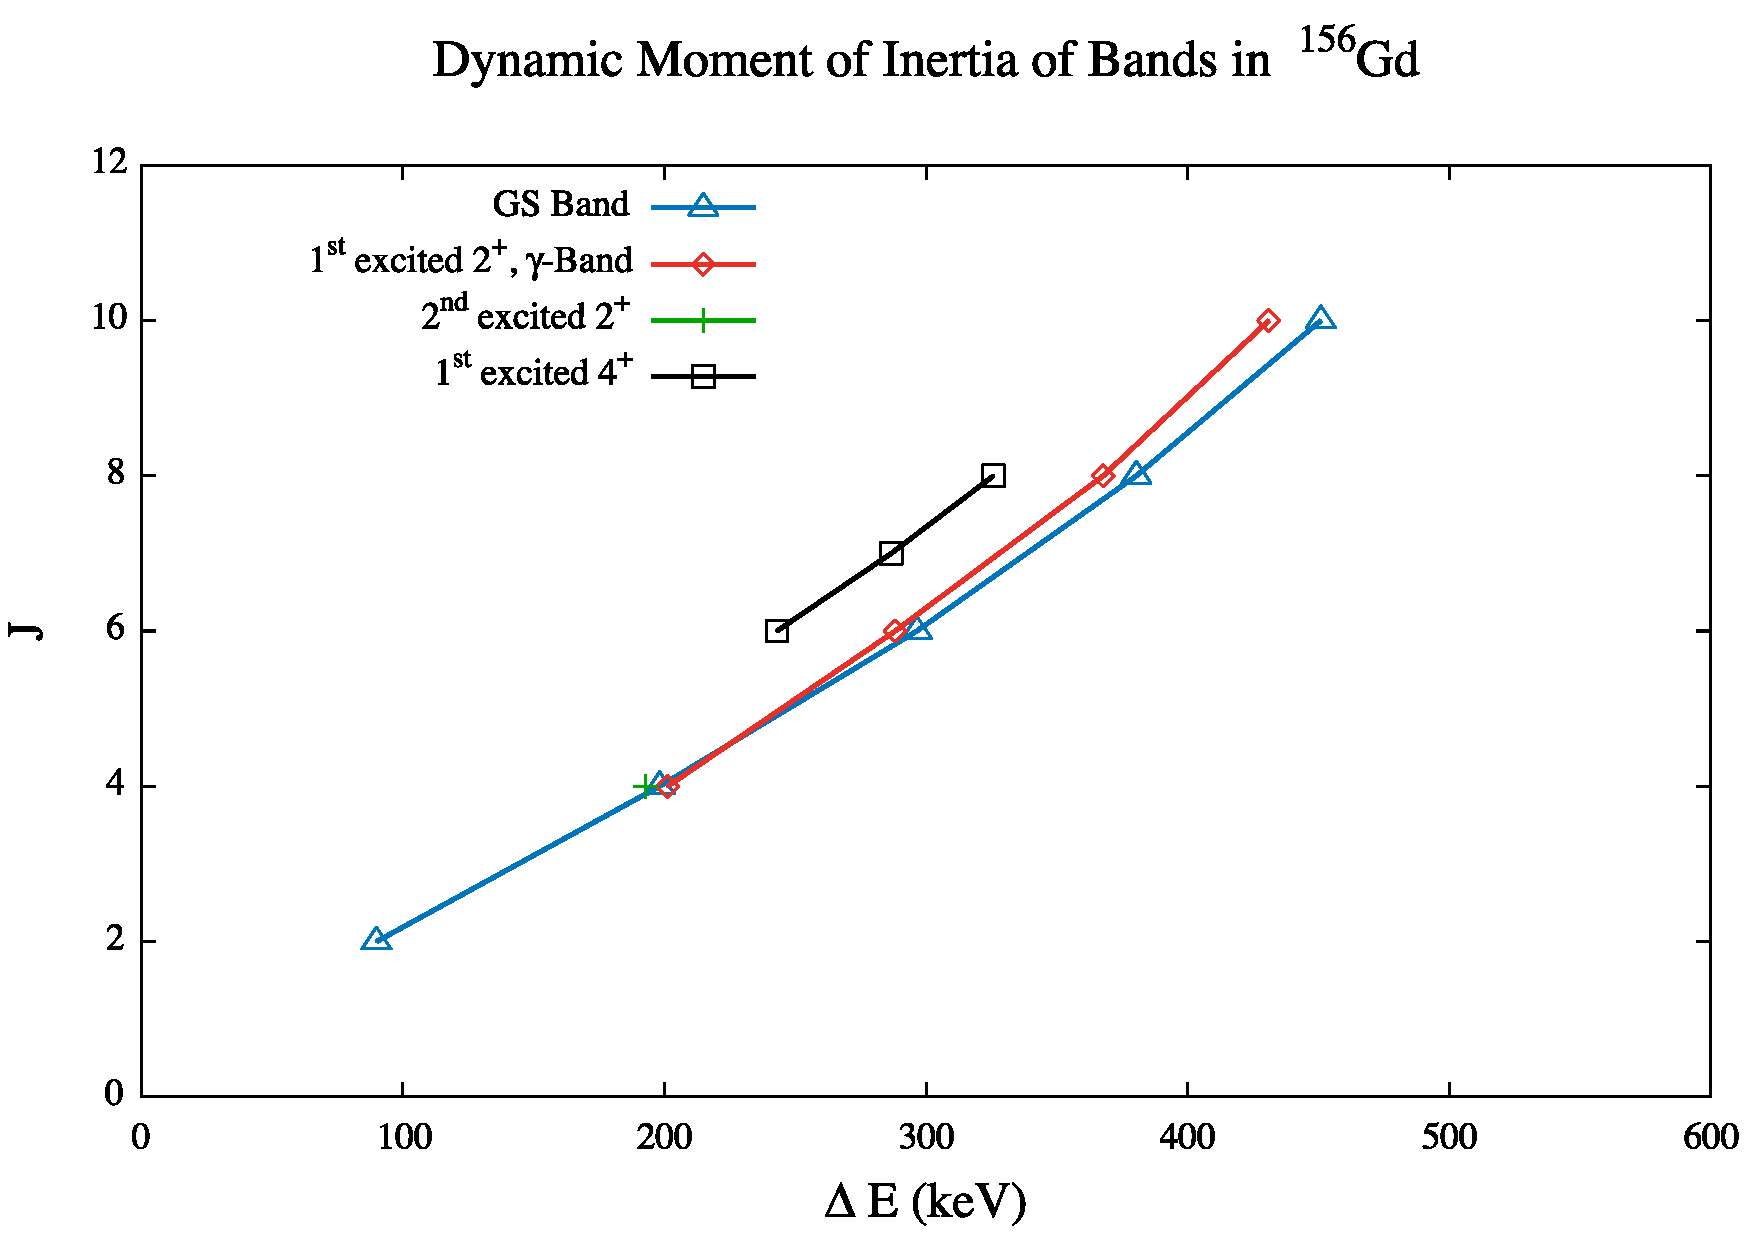
\includegraphics[scale=0.45]{Discussion/156_Dynamic.pdf}
    \caption{The dynamic moments of inertia of the non-$0^+$ bands seen in the experiment. As is seen visually and with the slopes, the ground state band and the $\gamma$ band have similar moments of inertia, and overlap within two standard deviations.}
    \label{fig:156_Dynamic}
\end{figure}

\begin{figure}[!]
    \centering
    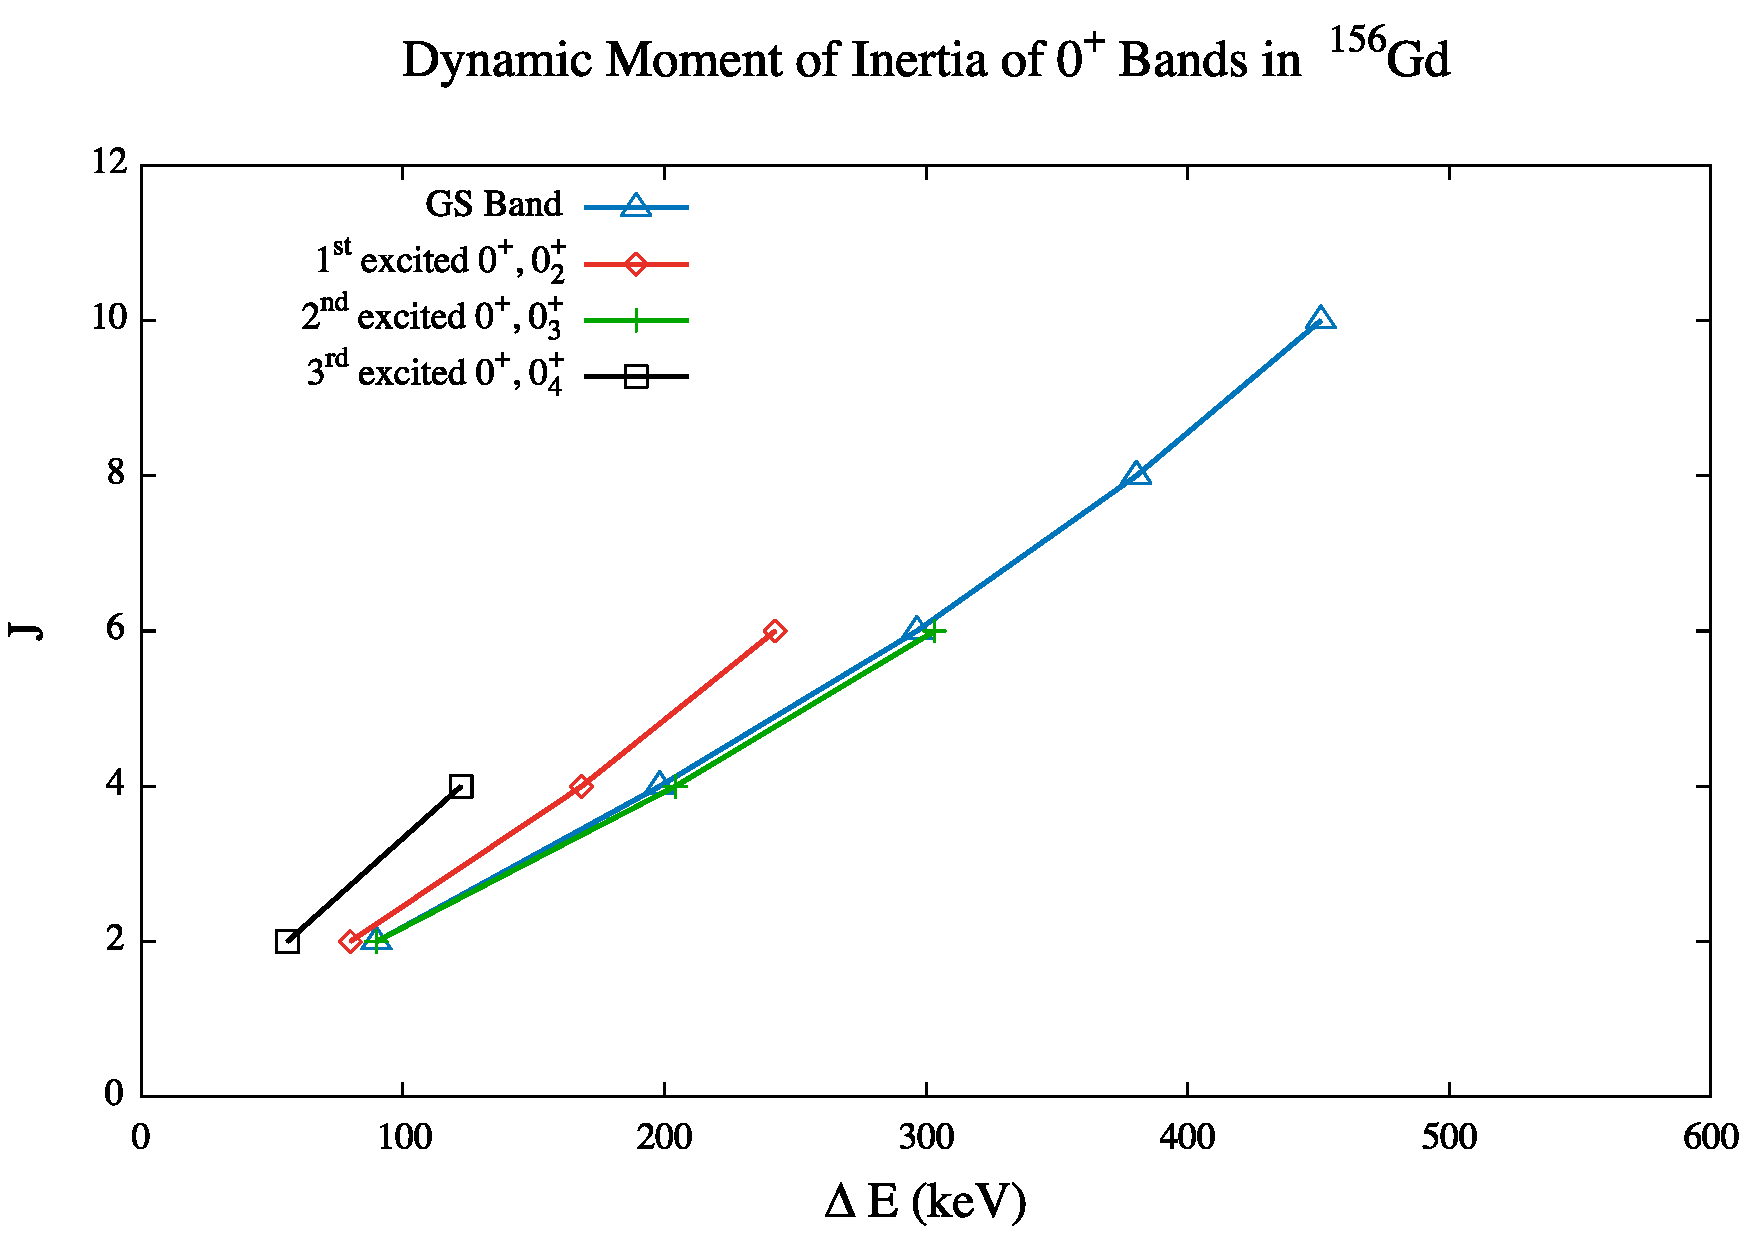
\includegraphics[scale=0.45]{Discussion/156_Dynamic0.pdf}
    \caption{The dynamic moments of inertia of the four $0^+$ bands seen in the experiment. As is seen visually and with the slopes, the ground state band and the first excited $0^+$ band have very similar moments of inertia.}
    \label{fig:156_Dynamic0}
\end{figure}

\begin{table}[!]
    \centering
    \caption{Dynamic Moments of Inertia of Bands seen in $^{156}$Gd}
    \begin{tabular}{c|c}
        \toprule
        Band & Moment of Inertia  \\
        \hline
        Ground State & 0.0220 (11) \\
        1st excited $0^+$, $0^+_2$ & 0.0245 (13) \\
        2nd excited $0^+$, $0^+_3$ & 0.0187 (8) \\
        3rd excited $0^+$, $0^+_4$ & 0.0301 \\
        1st excited $2^+$, $\gamma$-band & 0.0259 (13) \\
        1st excited $4^+$ & 0.0242 (10)  \\
        \bottomrule
    \end{tabular}
    \\[2pt]
    \footnotesize
    \label{tab:156_Dynamic}
    Table \ref{tab:156_Dynamic}: List of the moments of inertia of the bands seen in $^{156}$Gd in this experiment. The moment of inertia is the slope in a least-squares linear regression. Those without error only had one or two points of energy difference, so the standard deviation of the slope could not be calculated. The ground state band and the first excited $0^+$ band agree within two standard deviations. The same is true of the ground state band and both the $\gamma$-band and first excited $4^+$ band.
\end{table}

The $\gamma$-band, seen in Figure \ref{fig:156_Dynamic} is a vibration built on the ground state, leading to a nearly identical dynamic moment of inertia. The $K=4^+$ band has a nearly identical moment of inertia to the $\gamma$-band, indicating it, too, may be a vibration built on the same structure as the ground state. The first excited $0^+$ state, $0^+_2$, seen in Figure \ref{fig:156_Dynamic0}, agrees with the $\gamma$-band within $1\sigma$. The variation in the error of slopes has to do with the slow change in $\mathcal{J}^{(2)}$ due to the increase in spin. 

\subsection{$K^{\pi}=0^+_2$, First Excited $0^+$ Band, 1049.487 keV}

The conversion coefficients for the singles data originating from the first excited $0^+$ band are in Table \ref{tab:156Gd_Single_02_Disc}. The first excited $0^+$ band has a very similar slope to the ground state band, as seen both in Figure \ref{fig:156_Dynamic0} and Table \ref{tab:156_Dynamic}. The two bands agree within $2\sigma$. Without more statistics, data could not be collected for outgoing transitions from the first excited $0^+$ band.

This band is a good candidate for shape coexistence. It has a clearly differing dynamic moment of inertia from the ground state band, although it is similar to the $\gamma$ vibration band.

\begin{landscape}
    \begin{longtable}{>{\footnotesize}c|>{\footnotesize}c|>{\footnotesize}c|>{\footnotesize}c|>{\footnotesize}c|>{\footnotesize}c|>{\footnotesize}c|>{\footnotesize}c|>{\footnotesize}c|>{\footnotesize}c|>{\footnotesize}c}
    \caption{$^{156}$Gd $K_i=0^+_2$ Internal Conversion Coefficients from Singles}
        \label{tab:156Gd_Single_02_Disc}\\
    \toprule
$E$ (keV)	&	$J^{\pi}	\rightarrow	J^{\pi}$	&	$E_i$ (keV)	&	$E_f$ (keV)	&	Multipolarity	&	$\delta$	& Shell &	$\alpha$ (This Work)	&	$\alpha$  (Theory)\citep{kibedi08:_BRICC}	&	$\alpha$ (Konijn)\citep{konijn81:_156gd} &  $\epsilon^2$ (This Work)	\\
\hline		
\endfirsthead
    \caption[]{$^{156}$Gd $K_i=0^+_2$ Internal Conversion Coefficients from Singles}\\
    \toprule
$E$ (keV)	&	$J^{\pi}	\rightarrow	J^{\pi}$	&	$E_i$ (keV)	&	$E_f$ (keV)	&	Multipolarity	&	$\delta$ & Shell &	$\alpha$ (This Work)	&	$\alpha$  (Theory)\citep{kibedi08:_BRICC}	&	$\alpha$ (Konijn)\citep{konijn81:_156gd}	&  $\epsilon^2$ (This Work)\\
\hline		
\endhead
\endfoot
\multicolumn{11}{p{1.4\textwidth}}{Table \ref{tab:156Gd_Single_02_Disc}: A list of conversion coefficients from $^{156}$Gd, originating in the $K_i=0^+_2$ band.. Multipolarities and mixing ratios were taken from the nuclear date sheets\citep{reich12:_nds_156}. Unless otherwise stated, the $\alpha$ values are $\alpha_K$. An angular distribution correction has been applied based on multipolarities for pure transitions, and those with known mixing ratios. The first error is statistical, the second is systematic. Numbers are compared with Konijn et al\citep{konijn81:_156gd}. For transitions with an E0 component, the correction was applied assuming just the M1 and E2 components. The theory value is based on the listed multipolarity, also neglecting the E0 component in those cases. The $\epsilon^2$ values listed are for transitions with an E0 component possible, and a large enough $\alpha_{exp}$.}
\endlastfoot
1040.470	&	$2^+_{0^+_{2}}	\rightarrow	2^+_{gs}$	&	1129.437	&	88.970	&	E2+E0+M1	&	$-5.9^{+14}_{-28}$	& K &	0.0152 (10) (2)	&	0.0022 (1)	&	0.014 (3)	& $0.4187(275)^{+995}_{-1988}$\\ \hline
    \end{longtable}
\end{landscape}

\subsection{$K^{\pi}=0^+_3$, Second Excited $0^+$ Band, 1168.186 keV}

The conversion coefficients for the gated data originating from the second excited $0^+$ band are in Table \ref{tab:156Gd_03_Gate_Disc}. The second excited $0^+$ band could be seen going to both the $\gamma$ band and first excited $0^+$ band. It has a very different dynamic moment of inertia compared to those two. This change in shape may account for the large $\rho^2$ value between the first and second $0^+$ excited states, in Table \ref{tab:156Gd_E0}. In this data, transitions for the $2^+$ and $4^+$ states in this band were inconclusive about E0 components to the first excited $0^+$ state, and the $2^+$ state may have an E0 component to the $\gamma$-band. The $2^+$ and $4^+$ transitions examined do not have known mixing ratios, so $\alpha q^2$ can be found in \ref{tab:156Gd_E0}.

With the band's similarity in shape to the ground state band for the dynamic moment of inertia, this band is an excellent candidate to be the $\beta$-vibration. However, without conversion coefficients to the ground state band, this cannot be further explored.

\begin{landscape}
    \begin{longtable}{c|c|c|c|c|c|c|c|c|c}
        \caption{$J^{\pi}\rightarrow J^{\pi}$ Transitions for $K_i=0^+_3$ in $^{156}$Gd}
        \label{tab:156Gd_03_Gate_Disc}\\
        \toprule
        &	& & & 	&  &	& \multicolumn{2}{c|}{Theory\citep{kibedi08:_BRICC}}	\\
        $E_i$ (keV)	& $J^{\pi}_i$ &	$E_f$ (keV)	& Band &$E$ (keV)	&	Gate &		$\alpha$ (This Work)	& $\alpha$(M1) & $\alpha$(E2) & $\epsilon^2$ (This Work)\\
        \hline
        \endfirsthead
        \toprule
        \caption[]{$J^{\pi}\rightarrow J^{\pi}$ Transitions for $K_i=0^+_3$ in $^{156}$Gd}\\
        & & &	& 	&  &	& \multicolumn{2}{c|}{Theory\citep{kibedi08:_BRICC}}	\\
        $E_i$ (keV)	& $J^{\pi}_i$ &	$E_f$ (keV)	& $J^{\pi}_f$ &$E$ (keV)	&	Gate &		$\alpha$ (This Work)	& $\alpha$(M1) & $\alpha$(E2) & $\epsilon^2$ (This Work) \\
	    \endhead
	    \endfoot
	    \multicolumn{10}{p{1.4\textwidth}}{A list of conversion coefficients from $^{156}$Gd for $J^{\pi}\rightarrow J^{\pi}$ transitions for $K_i=0^+_3$ seen in the gated data. All listed theoretical values are for the K-shell internal conversion coefficient. The $\epsilon^2$ values listed are for transitions with a large enough $\alpha_{exp}$, and assumed to be pure E2 transitions, to give a minimum $\epsilon^2$,a lower limit. For $\alpha_{exp}$ that are upper limits, $\epsilon^2$ is not listed. No $\epsilon^2$ is indicated for the $0^+\rightarrow 0^+$ transitions. Numbers are compared with theoretical values for illustration. All coefficients are K-shell electrons. }
	    \endlastfoot
        1168.186 & $0^+_{3}$ & 1049.487  & $0^+_{2}$ & 118.71 &  960.50771 & $>1.1970$ & 1.042 (15) & 0.726 (11)\\
        \hline
        1258.075 & $2^+_{0^+_{3}}$ & 1129.437 & $2^+_{0^+_{2}}$ & 128.638 & 1040.470 & $>0.5325$ & 0.830 (12) & 0.578 (8)\\ \hline
        1258.075 & $2^+_{0^+_{3}}$ & 1154.152 & $2^+_{\gamma}$ & 103.92 & 1065.1781 & $>2.9695$ & 1.524 (22)  & 1.049 (15) & $>1.9205$\\ \hline
        1462.297 & $4^+_{0^+_{3}}$ & 1297.822 & $4^+_{0^+_{2}}$ & 164.469 & 1009.649 & $>0.4870$ & 0.416 (6) & 0.279 (4) & $>0.208$ \\ \hline
        1462.297 & $4^+_{0^+_{3}}$ & 1355.422 & $4^+_{\gamma}$ & 106.88 & 1067.2325 & $>0.7233$ & 1.405 (20) & 0.972 (14) \\ 
        \bottomrule
    \end{longtable}
\end{landscape}

\subsection{$K^{\pi}=2^+$, $\gamma$ Band, 1065.1781 keV}

The conversion coefficients for the singles data originating from the first excited $2^+$ band, the $\gamma$-vibrational band are in Table \ref{tab:156Gd_Single_02_Disc}. The $\gamma$ band has a very similar slope to the ground state band, as seen both in Figure \ref{fig:154_Dynamic0} and Table \ref{tab:156_Dynamic}, indicating similar moments of inertia, although the slope is higher than that seen by the ground state band or first excited $0^+$ band. The transitions between the first excited $0^+$ band and the $\gamma$ band are not energetically capable of conversion electrons for the $2^+_{\gamma}\rightarrow 2^+_{0^+_2}$ transition, and below the energy threshold of the detectors in this work for the $4^+_{\gamma}\rightarrow 4^+_{0^+_2}$ transition.

\begin{landscape}
    \begin{longtable}{>{\footnotesize}c|>{\footnotesize}c|>{\footnotesize}c|>{\footnotesize}c|>{\footnotesize}c|>{\footnotesize}c|>{\footnotesize}c|>{\footnotesize}c|>{\footnotesize}c|>{\footnotesize}c}
    \caption{$^{156}$Gd $K_i=2^+_1$, $\gamma$ Internal Conversion Coefficients from Singles}
        \label{tab:156Gd_Single_gamma_Disc}\\
    \toprule
$E$ (keV)	&	$J^{\pi}	\rightarrow	J^{\pi}$	&	$E_i$ (keV)	&	$E_f$ (keV)	&	$T_{1/2}$ (fs)	&	Multipolarity	& Shell &	$\alpha$ (This Work)	&	$\alpha$  (Th)	&	$\alpha$ (Konijn)	\\
\hline		
\endfirsthead
    \caption[]{$^{156}$Gd $K_i=2^+_1$, $\gamma$ Internal Conversion Coefficients from Singles}\\
    \toprule
$E$ (keV)	&	$J^{\pi}	\rightarrow	J^{\pi}$	&	$E_i$ (keV)	&	$E_f$ (keV)	&	$T_{1/2}$ (fs)	&	Multipolarity	& Shell &	$\alpha$ (This Work)	&	$\alpha$  (Th)	&	$\alpha$ (Konijn)	\\
\hline		
\endhead
\endfoot
\multicolumn{10}{p{1.4\textwidth}}{Table \ref{tab:156Gd_Single_gamma_disc}: A list of conversion coefficients from $^{156}$Gd, originating in the $K_i=2^+_1$, $\gamma$ band. Multipolarities and mixing ratios were taken from the nuclear date sheets\citep{reich12:_nds_156}. Unless otherwise stated, the $\alpha$ values are $\alpha_K$. An angular distribution correction has been applied based on multipolarities for pure transitions, and those with known mixing ratios. The first error is statistical, the second is systematic. Numbers are compared with Konijn et al\citep{konijn81:_156gd}.}
\endlastfoot
399.56	&	$9^+_{\gamma}	\rightarrow	7^+_{\gamma}$	&	2249.65	&	1849.84	&		&	E2	& K &	0.0077 (8) (3)	&	0.0205 (3)	&	0.026 (5)	\\ \hline
921.83	&	$5^+_{\gamma}	\rightarrow	6^+_{gs}$	&	1506.863	&	584.715	&	400	&	E2	& K &	0.0041 (9) (5) &	0.0028 (1)	&	0.0030 (7)	\\ \hline
1059.31	&	$6^+_{\gamma}	\rightarrow	6^+_{gs}$	&	1643.653	&	584.715	&		&	E2	& K &	0.0013 (5) (1)	&	0.0021 (1)	&	0.0013 (8)	\\ \bottomrule
    \end{longtable}
\end{landscape}

\subsection{$K^{\pi}=2^+$, Second Excited $2^+$ Band, 1827.841 keV}

The conversion coefficients for the gated data originating from the second excited $2^+$ band are in Table \ref{tab:156Gd_22_Gate_Disc}. The second excited $2^+$ band has a smaller slope than the ground state band, first excited $0^+$ band and the $\gamma$ band. The moment of intertia could not be determined as there were not enough known states in the band. Transitions to the $0^+_3$ band do not indicate an E0 component. Transitions to the first excited $0^+$ band and the $\gamma$ band may have an E0 component, but with only upper limits, it is inconclusive. These limits indicate approximately equal strengths to both bands, as seen in Table \ref{tab:156Gd_BE0_Comp}, a possible indication it may be a mix of the two bands. The transitions examined do not have known mixing ratios, so $\alpha q^2$ can be found in \ref{tab:156Gd_E0}.

\begin{landscape}
    \begin{longtable}{c|c|c|c|c|c|c|c|c|c}
        \caption{$J^{\pi}\rightarrow J^{\pi}$ Transitions for $K_i=2^+_2$ in $^{156}$Gd}
        \label{tab:156Gd_22_Gate_Disc}\\
        \toprule
        &	& & & 	&  &	& \multicolumn{2}{c|}{Theory}	\\
        $E_i$ (keV)	& $J^{\pi}_i$ &	$E_f$ (keV)	& Band &$E$ (keV)	&	Gate &		$\alpha$ (This Work)	& $\alpha$(M1) & $\alpha$(E2)&	$\alpha$ (Konijn)	\\
        \hline
        \endfirsthead
        \toprule
        \caption[]{$J^{\pi}\rightarrow J^{\pi}$ Transitions for $K_i=2^+_2$ in $^{156}$Gd}\\
        & & &	& 	&  &	& \multicolumn{2}{c|}{Theory}	\\
        $E_i$ (keV)	& $J^{\pi}_i$ &	$E_f$ (keV)	& $J^{\pi}_f$ &$E$ (keV)	&	Gate &		$\alpha$ (This Work)	& $\alpha$(M1) & $\alpha$(E2)&	$\alpha$ (Konijn)	 \\
	    \endhead
	    \endfoot
	    \multicolumn{10}{p{1.4\textwidth}}{A list of conversion coefficients from $^{156}$Gd for $J^{\pi}\rightarrow J^{\pi}$ transitions for $K_i=2^+_2$ seen in the gated data. All listed theoretical values are for the K-shell internal conversion coefficient. Numbers are compared with theoretical values for illustration. All coefficients are K-shell electrons. }
	    \endlastfoot
        1827.841 & $2^+_{2^+_2}$ & 1129.437 & $2^+_{0^+_{2}}$ & 698.407 & 1040.470 & $<0.0208$ & 0.00932 (13) & 0.00506 (7) & \\ \hline
        1827.841 & $2^+_{2^+_2}$ & 1154.152 & $2^+_{\gamma}$ & 673.684 & 1065.1781 & $<0.0228$ & 0.01018 (15) & 0.00550 (8) &\\ \hline
        1827.841 & $2^+_{2^+_2}$ & 1258.075 & $2^+_{0^+_{3}}$ & 569.771 & 1169.087 & $<0.0013$ & 0.01545 (22) & 0.00819 (12) & 0.006 (4) \\
        \bottomrule
    \end{longtable}
\end{landscape}

\subsection{$K^{\pi}=4^+$, First Excited $4^+$ Band, 1510.594 keV}

The conversion coefficients for the singles and gated data originating from the first excited $4^+$ band are in Tables \ref{tab:156Gd_Single_41_Disc} and \ref{tab:156Gd_41_Gate_Disc}, respectively. Only the first state in the first excited $4^+$ band was able to get electron spectroscopy. This band has a similar slope to the ground state band, first excited $0^+$ band and the $\gamma$ band, although it is least like the ground state band dynamic moment of inertia. The lower limits on the conversion coefficients to the first excited $0^+$ band and the $\gamma$ band tell very little, as all forms of multipolarity, including a pure E2, are still accessible. The transitions examined do not have known mixing ratios, so $\alpha q^2$ can be found in \ref{tab:156Gd_E0}.

The low limits of the conversion coefficients indicate this could well be the $4^+$ component of the $\gamma-\gamma$ vibration. The dynamic moment of inertia supports this interpretation.

\begin{landscape}
    \begin{longtable}{c|c|c|c|c|c|c|c|c}
    \caption{$^{156}$Gd $K_i=4^+_1$ Internal Conversion Coefficients from Singles}
        \label{tab:156Gd_Single_41_Disc}\\
    \toprule
$E$ (keV)	&	$J^{\pi}	\rightarrow	J^{\pi}$	&	$E_i$ (keV)	&	$E_f$ (keV)	&	$T_{1/2}$ (fs)	&	Multipolarity	& Shell &	$\alpha$ (This Work)	&	$\alpha$  (Theory)\citep{kibedi08:_BRICC}		\\
\hline		
\endfirsthead
    \caption[]{$^{156}$Gd $K_i=2^+_1$, $\gamma$ Internal Conversion Coefficients from Singles}\\
    \toprule
$E$ (keV)	&	$J^{\pi}	\rightarrow	J^{\pi}$	&	$E_i$ (keV)	&	$E_f$ (keV)	&	$T_{1/2}$ (fs)	&	Multipolarity	& Shell &	$\alpha$ (This Work)	&	$\alpha$  (Theory)\citep{kibedi08:_BRICC}\\
\hline		
\endhead
\endfoot
\multicolumn{9}{p{1.4\textwidth}}{Table \ref{tab:156Gd_Single_41_Disc}: A list of conversion coefficients from $^{156}$Gd, originating in the $K_i=4^+_1$ band. Multipolarities and mixing ratios were taken from the nuclear data sheets\citep{reich12:_nds_156}. Unless otherwise stated, the $\alpha$ values are $\alpha_K$. An angular distribution correction has been applied based on multipolarities for pure transitions, and those with known mixing ratios. The first error is statistical, the second is systematic.}
\endlastfoot
355.87	&	$4^+_{4^+}	\rightarrow	2^+_{\gamma}$	&	1510.594	&	1154.152	&	189000	&	E2	& K &	0.0206 (8) (7)	&	0.0281 (4)	\\ \bottomrule
    \end{longtable}
\end{landscape}

\begin{landscape}
    \begin{longtable}{c|c|c|c|c|c|c|c|c}
        \caption{$J^{\pi}\rightarrow J^{\pi}$ Transitions for $K_i=4^+_1$ in $^{156}$Gd}
        \label{tab:156Gd_41_Gate_Disc}\\
        \toprule
        &	& & & 	&  &	& \multicolumn{2}{c}{Theory\citep{kibedi08:_BRICC}}	\\
        $E_i$ (keV)	& $J^{\pi}_i$ &	$E_f$ (keV)	& $J^{\pi}_f$ & $E$ (keV)	&	Gate &		$\alpha$ (This Work)	& $\alpha$(M1) & $\alpha$(E2)\\
        \hline
        \endfirsthead
        \toprule
        \caption[]{$J^{\pi}\rightarrow J^{\pi}$ Transitions for $K_i=4^+_1$ in $^{156}$Gd}\\
        & & &	& 	&  &	& \multicolumn{2}{c}{Theory\citep{kibedi08:_BRICC}}	\\
        $E_i$ (keV)	& $J^{\pi}_i$ &	$E_f$ (keV)	& $J^{\pi}_f$ &$E$ (keV)	&	Gate &		$\alpha$ (This Work)	& $\alpha$(M1) & $\alpha$(E2) \\
	    \endhead
	    \endfoot
	    \multicolumn{9}{p{1.4\textwidth}}{A list of conversion coefficients from $^{156}$Gd for $J^{\pi}\rightarrow J^{\pi}$ transitions for $K_i=4^+_1$ seen in the gated data. All listed theoretical values are for the K-shell internal conversion coefficient. Numbers are compared with theoretical values for illustration. All coefficients are K-shell electrons. }
	    \endlastfoot
        1510.594 & $4^+_{4^+_1}$ &1297.822 & $4^+_{0^+_{3}}$ & 212.771 & 1009.649 & $>0.0704$  & 0.204 (3) & 0.1282 (18) \\ \hline
        1510.594 & $4^+_{4^+_1}$ & 1355.422 & $4^+_{\gamma}$ & 155.168 & 1067.2325 & $>0.0981$ & 0.490 (7) & 0.333 (5)  \\
        \bottomrule
    \end{longtable}
\end{landscape}

\subsection{Summary and Conclusions}

Table \ref{tab:156gd_summary} contains a summary of relevant data for the $0^+$ states in $^{156}$Gd. For the low-lying levels, there is a good amount of information known. The cross sections from $(p,t)$ are from Fleming et al.\citep{fleming73:_156gd}. These measurements were done in 1973, and are the most recent $(p,t)$ measurements for $^{156}$Gd. With new high-precision spectroscopy and the discovery of so many $0^+$ states in the rare-earth region, this nucleus should be revisited via the reaction.

The conversion coefficients combined with the dynamic moments of inertia for these bands allows for the interpretation of the nature of these bands. The $0^+_2$ band  is a good candidate for shape coexistence. The $0^+_3$ band has indications of being the $\beta$-vibration. From the common interpretation of the $2^+_1$ band as the $\gamma$-vibration,  $4^+_1$ band may to be one of the two components of the $\gamma-\gamma$ two phonon vibration. The $2^+_2$ band cannot be interpreted at this time.

\begin{table}
    \centering
\begin{threeparttable}
    \centering
    \caption{Summary of $0^+$ State Information in $^{156}$Gd}
    \label{tab:156gd_summary}
    \begin{tabular}{c|c|c|c}
        E (keV) & $(p,t)$ ($\mu$b/sr) & $\tau$ (ps)\citep{aprahamian18:_156gd} & Conv. Elec \\
        \toprule
        0.0 & 624 & Stable & Ground State \\
        1049.487(2) & 64 & $1.81<\tau<4.75$ & $\times$ \\
        1168.186(7) & 12 & $3.00<\tau<14.7$ &  $\times$ \\
        1715.211(4) &  & $0.02<\tau<7.08$ & $\times$ \\
        1851.278(7) &  & & \\
        1988.5(2) &  & &  \\
        2082.0 &  & &  \\
        \bottomrule
    \end{tabular}
    \begin{tablenotes}[para]
        Table \ref{tab:156gd_summary}: The current state of information for the $0^+$ states in $^{156}$Gd. The $(p,t)$ cross section is the $30\textdegree$ from Fleming et al.\citep{fleming73:_156gd}. The lifetimes are from Aprahamian et al.\citep{aprahamian18:_156gd}. Conversion electron measurements are from this work, B{\"a}cklin et al.\citep{backlin82:_156Gd}, Yamada et al.\citep{yamada76:_156gd}, Ewan et al.\citep{ewan62:_156gd}, and Peek et al.\citep{Peek64:_156gd}.
    \end{tablenotes}
\end{threeparttable}
\end{table}